% ESOP 2027 anonymous research-paper submission, Springer LNCS format.
% ESOP 2027 research submissions have no page limit.
% Camera-ready: 25 pages excluding bibliography; see README.md.
\documentclass[runningheads]{llncs}

\usepackage[T1]{fontenc}
\usepackage{graphicx}
% Explicit dependencies formerly supplied by acmart.
\usepackage[dvipsnames]{xcolor}
\usepackage{amsmath}
\usepackage{amssymb}
\usepackage{stmaryrd}
%\usepackage{amsthm}
\usepackage{mathtools}
\DeclarePairedDelimiter\abs{\lvert}{\rvert}
\usepackage{mdframed}
\usepackage{booktabs}
\usepackage{tabularx}
\usepackage{tikz}
\usepackage{csquotes}
\usetikzlibrary{patterns,shapes,positioning,automata}
\usepackage[altpo]{backnaur}
\usepackage[shortlabels]{enumitem}
\usepackage{multicol}
\usepackage{adjustbox}
\usepackage{wrapfig}
\usepackage{placeins}
\usepackage{nicefrac}
\usepackage{makecell}
\usepackage{siunitx}
\usepackage{colortbl}
\usepackage{listings}
\usepackage{thmtools}
\usepackage{thm-restate}
% LNCS proof environments do not insert an end-of-proof symbol automatically.
\usepackage{etoolbox}
\AtEndEnvironment{proof}{\qed}
\usepackage{bussproofs}
\usepackage{xspace}
\usepackage{pifont}
% Suppress author-identifying draft comments in the anonymous submission.
% Remove "disable" only for an internal working copy.
\usepackage[disable,textsize=scriptsize,bordercolor=white]{todonotes}
\usepackage{setspace}
\usepackage[hidelinks]{hyperref}
\hypersetup{pdfauthor={}}
\usepackage{cleveref}


% colors
\newcommand{\blue}[1]{\textcolor{blue}{#1}}
\newcommand{\red}[1]{\textcolor{Bittersweet}{#1}}
\newcommand{\gray}[1]{\textcolor{gray}{#1}}

%Preliminaries
\newcommand{\weight}[1]{|#1|}
\newcommand{\nweight}[1]{|#1|_{\prsqbrackop\prsqbrackcl}}
\newcommand{\subdists}{{\Deltasub \Sigma}}
\newcommand{\subdist}[1]{{\Deltasub #1}}
\newcommand{\subhalfdists}{{\Deltasubhalf \Sigma}}
\newcommand{\dists}{{\Delta \Sigma}}
\newcommand{\onlybdists}{\langle \bool \rangle}%Not used everywhere in the document
\newcommand{\onlynbdists}{\langle \neg \bool \rangle}%Not used everywhere in the document
\newcommand{\Deltasub}{\Delta_{\leq 1}}
\newcommand{\Deltasubhalf}{\Delta_{\leq 0.5}}
\newcommand{\Deltaspec}[1]{\Delta_{#1}}%Delta Speciale. (rarely used)
\newcommand{\statevals}{\textnormal{E}}
\newcommand{\LFPstateval}{e}
\newcommand{\LFPset}{X}%For the reach transformer
\newcommand{\LFPhoset}{X}%For the pre transformer: higher order
\newcommand{\Mfdr}{\initSet_{\textsc{fdr}}}
\newcommand{\varsfdr}{\vars_{\textsc{fdr}}}
\newcommand{\Mfldr}{\initSet_{\textsc{fldr}}}
\newcommand{\varsfldr}{\vars_\textsc{fldr}}
\newcommand{\stratsfdr}{\Pi^{\epsilon}_{\textsc{fdr}}}
\newcommand{\modelst}{\models_t}
\newcommand{\modelsp}{\models_p}
\newcommand{\initDist}{\mu_0} %Not used everywhere in the document?
\newcommand{\initStateVal}{\mu_0} %Not used everywhere in the document?
\newcommand{\initSet}{M} 
\newcommand{\postSet}{M} %FOR THE PRE TRANSFORMER
\newcommand{\statevalSet}{M} %Only once used
\newcommand{\hSetOne}{M} %hoare Sets (=(sub)-distribution sets)
\newcommand{\hSetTwo}{N}
\newcommand{\hSetThree}{O}
\newcommand{\hSetFour}{P}
\newcommand{\triple}[3]{\{\hspace{-2.1pt}|#1|\hspace{-2.1pt}\}~#2~\{\hspace{-2.1pt}|#3|\hspace{-2.1pt}\}} % braces could be improved
\newcommand{\tripleGen}{\triple{\hSetOne}{\prog}{\hSetTwo}} % generic triple
\newcommand{\inv}{I}
\newcommand{\statesSet}[4]{S_{\progvar{#1} \rightarrow #2}^{\progvar{#3} \rightarrow #4}}%WIRD auch für nur 2 Argumente Ohne Makro im Dokument verwendet
\newcommand{\marg}[2]{\mathbb{M}_{#1}(#2)}
\newcommand{\fixation}[3]{\mathbb{F}_{#1 \rightarrow #2 \sim #3}}
\newcommand{\unif}[3]{\mathsf{unif}_{#1}(#2,\dots,#3)}
\newcommand{\unifeps}[3]{\mathsf{unif}_{#1}^{\pm\epsilon}(#2,\dots,#3)}
\newcommand{\pro}[3]{\textnormal{Pr}_{#1}(#2 \mapsto #3)}
\newcommand{\prosim}[4]{\textnormal{Pr}_{#1}[#2 #3 #4]}
\newcommand{\diff}[1]{\textnormal{diff}(#1)}
\newcommand{\diffn}[2]{\textnormal{diff}_{#1}^{#2}}
\newcommand{\pr}[2]{\textnormal{Pr}_{#1}[#2]}
\newcommand{\minim}[2]{\min\{#1, #2\}}%Minimum
\newcommand{\dirac}[1]{\delta_{#1}} % Dirac distribution over state #1


%Conventional Letters
\newcommand{\prog}{C}
\newcommand{\loopbody}{B}
\newcommand{\progZero}{\prog_0}
\newcommand{\progOne}{\prog_1}
\newcommand{\progTwo}{\prog_2}
\newcommand{\progThree}{\prog_3}
\newcommand{\progFour}{\prog_4}
\newcommand{\arith}{E}
\newcommand{\bool}{\varphi}
\newcommand{\probability}{p}
\newcommand{\textvar}[1]{\normalfont #1}%Program variables IN TEXTS. That means when either only "variable v is..." occurs in text or VERY short math thins like "(v,c) is..." In longer math equations or "\sigma(v)..." always progvar macro is used. In lstlisting outside of math mode annotations, nothing is used.
\newcommand{\progvar}[1]{#1}%Program variables
\newcommand{\numb}[1]{\mathbf{#1}}%VALUES of IDENTICAL NAMES prog vars
\newcommand{\supp}{\textnormal{supp}}
\newcommand{\pgcl}{\textnormal{pGCL}}
\newcommand{\loops}{\textnormal{Loop}}
\newcommand{\pgclwhile}{\abs{\pgcl}_{\textnormal{while}}}
\newcommand{\progwhile}[1]{\abs{#1}_{\textnormal{while}}}
\newcommand{\conf}{\textnormal{Conf}}

%Einfache Namen
\newcommand{\vars}{\mathit{Var}}
\newcommand{\false}{\mathsf{f}}
\newcommand{\true}{\mathsf{t}}
\newcommand{\bools}{\mathbb{B}}
\newcommand{\Ifdr}{I^{\epsilon}_{\textsc{fdr}}}
\newcommand{\Ifldr}{I_{\textsc{fldr}}}
\newcommand{\Inim}{I_{\textsc{nim}}}
\newcommand{\progfldr}{\mathit{\prog_\textsc{fldr}}}
\newcommand{\progfdr}{\mathit{\prog_\textsc{fdr}}}
\newcommand{\prob}[2]{\textnormal{prob}_{#1}(#2)}
\newcommand{\probt}[2]{\textnormal{probt}_{#1}(#2)}
\newcommand{\prep}{\textnormal{prep}}
\newcommand{\lfp}{\mathsf{lfp\,}}
\newcommand{\nats}{\mathbb{N}}
\newcommand{\RgeqZero}{\mathbb{R}_{\geq 0}}
\newcommand{\RgeqZeroInf}{\mathbb{R}^{\infty}_{\geq 0}}
\newcommand{\RgZeroInf}{\mathbb{R}^{\infty}_{> 0}}
\newcommand{\supr}{\textnormal{sup}}
\newcommand{\infimum}{\textnormal{inf}}
\newcommand{\unmod}[1]{\textnormal{unmod}(#1)}

%Transformer
\newcommand{\reach}[1]{\mathsf{reach}\llbracket #1\rrbracket}
\newcommand{\post}[1]{\den{#1}} % Legacy name for the same semantics
\newcommand{\den}[1]{\mathsf{D}\llbracket #1\rrbracket}
\renewcommand{\wp}[1]{\textnormal{pre}\llbracket #1\rrbracket} %Should be the same, just old and new macro
\newcommand{\pre}[1]{\textnormal{pre}\llbracket #1\rrbracket} %Should be the same, just old and new macro


%n for normal: für wenn du die Namen der Transformer im Text benutzen möchtest
\newcommand{\reachn}{\mathsf{reach}}
\newcommand{\postn}{\denn}
\newcommand{\postcupn}{\mathsf{sp}^{\cup}}
\newcommand{\denn}{\mathsf{D}}
\newcommand{\wpn}{\textnormal{pre}} %Should be the same, just old and new macro
\newcommand{\pren}{\textnormal{pre}} %Should be the same, just old and new macro



%Inductive program structure
% UPPER CASE VERSION ARE SYNTAX FRAGMENTS TO BE USED IN ALIGN
\newcommand{\prfont}[1]{\textnormal{\texttt{#1}}}
\newcommand{\prspace}{\,}
\newcommand{\prparenop}{\prfont{(}}
\newcommand{\prparencl}{\prfont{)}}
\newcommand{\prsqbrackop}{\prfont{[}}
\newcommand{\prsqbrackcl}{\prfont{]}}
\newcommand{\prbraceop}{\prfont{\{}}
\newcommand{\prbracecl}{\prfont{\}}}
\newcommand{\ski}{\prfont{skip}}
\newcommand{\ass}[2]{#1\prspace\prfont{:=}\prspace#2}
\newcommand{\pchoice}[3]{\prbraceop#1\prbracecl \prspace \prsqbrackop#2\prsqbrackcl \prspace \prbraceop#3\prbracecl}
\newcommand{\nchoice}[2]{\{#1\} \prsqbrackop\prsqbrackcl \{#2\}}
\newcommand{\nchoicebox}{\prsqbrackop\prsqbrackcl}
\newcommand{\comp}[2]{#1\prspace\prfont{;}\prspace#2}
\newcommand{\SEMICLN}{\prspace\prfont{;}\prspace}
\newcommand{\ifelse}[3]{\prfont{if}\prspace\prparenop#1\prparencl\prspace\prbraceop#2\prbracecl\prspace\prfont{else}\prspace\prbraceop#3\prbracecl}
\newcommand{\ifelseskip}[2]{\prfont{if}\prspace\prparenop#1\prparencl\prspace\prbraceop#2\prbracecl}
\newcommand{\ELSE}{\prbracecl\prspace\prfont{else}\prspace\prbraceop}
\newcommand{\IF}[1]{\prfont{if}\prspace\prparenop#1\prparencl\prspace\prbraceop}
\newcommand{\while}[2]{\prfont{while}\prspace\prparenop#1\prparencl\prspace\prbraceop#2\prbracecl}
\newcommand{\WHILE}[1]{\prfont{while}\prspace\prparenop#1\prparencl\prspace\prbraceop}


%Preprocessing FLDR
\renewcommand{\H}[2]{H[#1,#2]}
\newcommand{\bound}[2]{\phi_{#1}(#2)}
\newcommand{\isThere}[2]{\Theta_{#1}(#2)}

%Shorthand Notation for Transformer Tables
%\newcommand{\postass}[2]{\overset{\rightharpoonup}{\ass{#1}{#2}}}
%\newcommand{\postass}[2]{\xrightharpoonup[\ass{#1}{#2}]{}}
%\newcommand{\preass}[2]{\xleftharpoonup[\ass{#1}{#2}]{}}
%\xrightharpoonup[below]{above}
\newcommand{\postass}[2]{\overset{\rightharpoonup}{\ass{#1}{#2}}}
\newcommand{\preass}[2]{\overset{\leftharpoonup}{\ass{#1}{#2}}}

\newcommand{\cl}[1]{\mathcal{M}_{#1}}%CLOSURE FOR BOOLS FOR PRE TRANSFORMER
\newcommand{\idSubDists}{\textnormal{id}_{2^{\subdists}}}

\newcommand{\clos}{c\ell}%CLOSURE FOR HOARE NEW WHILE RULES
\newcommand{\closOf}[1]{{\clos\,#1}}
\newcommand{\infW}[1]{\textnormal{Inf}_{\textnormal{w}}(#1)}%CLOSURE FOR HOARE NEW WHILE RULES
\newcommand{\closast}{\Delta_{\geq \infW{\inv}} \Sigma \cap \clos}
\newcommand{\closastinv}[1]{\Delta_{\geq \infW{#1}} \Sigma \cap \clos}%FOR SPECIFYING THE INV



%MDP Translation Stuff
\newcommand{\mdp}{\mathcal{M}}
\newcommand{\mdpTr}{\mdp_{\prog}}
%\newcommand{\strat}{\sigma} THIS IS NOW FOR PROGRAM STRATEGIES
\newcommand{\mdptuple}{(\states,\act,\prmdp)}
\newcommand{\states}{S}
\newcommand{\act}{{Act}}
\newcommand{\prmdp}{P}
\newcommand{\distsStates}{\Delta \states}
\newcommand{\subdistsStates}{\Deltasub \states}
\newcommand{\mdpDist}{\eta}
\newcommand{\mdpInitDist}{\eta_0}
\newcommand{\mdpInitDistTr}{\eta_{\initDist}}
\newcommand{\mdpInv}{\inv_{\mdp}}
\newcommand{\smallstep}[2]{\overset{#1.#2}{\longrightarrow}}
\newcommand{\bigstep}[1]{\overset{#1}{\rightsquigarrow}}
\newcommand{\bigstepn}{\rightsquigarrow}
\newcommand{\nextdist}[1]{#1}

%Markov Chains:
\newcommand{\markc}{\mathcal{M}}
\newcommand{\markctuple}{(\states,\prmdp)}
\newcommand{\markcTr}{\markc_{\prog}}

% from Tobi (intro)
\newcommand{\htrip}[3]{\blue{\{\hspace{-2.1pt}|#1|\hspace{-2.1pt}\}}~#2~\blue{\{\hspace{-2.1pt}|#3|\hspace{-2.1pt}\}}}
\newcommand{\intropre}{pre}
\newcommand{\intropost}{post}


\newcommand{\splitStateInline}[2]{\tikz[baseline=-2.75pt] \node [circle split,draw,rotate=90,inner sep=0.5pt] {\rotatebox{-90}{\tiny$#1$} \nodepart{lower} \rotatebox{-90}{\tiny$#2$}};}

% program annotation
\newcommand{\progAnno}[1]{\blue{\prfont{/\!\!/}~#1}}
\newcommand{\progAnnoNoSlashes}[1]{\blue{\textcolor{white}{\prfont{/\!\!/}}~#1}}

% space stuff
\newcommand{\eeq}{~{}={}~}
\newcommand{\iiff}{~{}\iff{}~}
\newcommand{\lland}{~{}\land{}~}



%Nondeterministic Choice Stuff
\newcommand{\lef}{l}
\newcommand{\rig}{r}
\newcommand{\progstrat}{\prog^{\strat}}
\newcommand{\denstrat}[1]{\mathsf{D}^{\strat}\llbracket #1\rrbracket}
\newcommand{\dens}[2]{\mathsf{D}^{#1}\llbracket #2\rrbracket}
\newcommand{\denhelper}[1]{\mathsf{H}^{\strat}\llbracket #1\rrbracket}
\newcommand{\denhelpernormal}{\mathsf{H}^{\strat}}
\newcommand{\denhelperf}[1]{\mathsf{F}^{\strat}\llbracket #1\rrbracket}
\newcommand{\denhelperfnormal}{\mathsf{F}^{\strat}}
\newcommand{\reachstrat}[1]{\mathsf{reach}^{\strat}\llbracket #1\rrbracket}
\newcommand{\poststrat}[1]{\mathsf{sp}^{\strat}\llbracket #1\rrbracket}
\newcommand{\posts}[2]{\mathsf{sp}^{#1}\llbracket #2\rrbracket}
\newcommand{\postcup}[1]{\mathsf{sp}^{\cup}\llbracket #1\rrbracket}
\newcommand{\postcap}[1]{\mathsf{sp}^{\cap}\llbracket #1\rrbracket}
\newcommand{\postall}[1]{\mathsf{sp}^{\forall}\llbracket #1\rrbracket}
\newcommand{\reachall}[1]{\mathsf{reach}^{\cup}\llbracket #1\rrbracket}
\newcommand{\strats}{\Pi}
\newcommand{\strat}{\pi}
\newcommand{\modelscup}{\models^{\cup}}
\newcommand{\postpi}[3]{\mathsf{sp}^{#1}_{#2}\llbracket #3\rrbracket}
\newcommand{\postmu}[3]{\mathsf{sp}^{#1}_{#2}\llbracket #3\rrbracket}

\newcommand{\stratsD}{\Pi}
\newcommand{\stratsMem}{\Pi_{\textnormal{Mem}}}
\newcommand{\stratsSigD}{\Pi_{\Sigma}}
\newcommand{\stratsN}{\Pi^{\Delta}}
\newcommand{\stratsSigN}{\Pi_{\Sigma}^{\Delta}}
\newcommand{\stratsSigNLC}{{}^{LC}\Pi_{\Sigma}^{\Delta}}
\newcommand{\stratsSigsD}{\Pi_{\Sigma^*}}
\newcommand{\stratsSigsN}{\Pi_{\Sigma^*}^{\Delta}}
\newcommand{\stratsCSigsD}{\Pi_{(\prog, \Sigma)^*}}
\newcommand{\stratsCSigsN}{\Pi_{(\prog, \Sigma)^*}^{\Delta}}
\newcommand{\stratsDeq}{{}^{=}\Pi}
\newcommand{\stratsSigDeq}{{}^{=}\Pi_{\Sigma}}
\newcommand{\stratsNeq}{{}^{=}\Pi^{\Delta}}
\newcommand{\stratsSigNeq}{{}^{=}\Pi_{\Sigma}^{\Delta}}
\newcommand{\stratsSigsDeq}{{}^{=}\Pi_{\Sigma^*}}
\newcommand{\stratsSigsNeq}{{}^{=}\Pi_{\Sigma^*}^{\Delta}}
\newcommand{\stratsCSigsDeq}{{}^{=}\Pi_{(\prog, \Sigma)^*}}
\newcommand{\stratsCSigsNeq}{{}^{=}\Pi_{(\prog, \Sigma)^*}^{\Delta}}
\newcommand{\stratsall}{\Pi^*}
\newcommand{\resprog}{\downharpoonright_{\sigma}}
\newcommand{\weaker}{\triangleright}
\newcommand{\loopc}{\textnormal{LC}}


%MDP Strategies
\newcommand{\tstrat}[1]{\mathfrak{S}_{#1}} %MDP strat that got translated from a (program) strat



%Nim Game
\newcommand{\Mnim}{\initSet_{\textsc{nim}}}
\newcommand{\prognim}{\mathit{\prog_\textsc{nim}}}
\newcommand{\stratnim}{\strat_{\textsc{nim}}}

%Tool names (used in related work)
\newcommand{\toolzar}{\textsf{Zar}\xspace}
\newcommand{\toolpsi}{\textsf{PSI}\xspace}

% wp shorthand in related work
\providecommand{\wpRelWork}{\wpn}



%New Commands
\newcommand{\Mhh}{\textnormal{Mhh}}
\newcommand{\idx}{\textnormal{idx}}
\newcommand{\proghh}{\textnormal{proghh}}
\newcommand{\Succ}{\textnormal{Succ}}

% Include sections and subsections in the PDF navigation without printing a TOC.
\setcounter{tocdepth}{2}

\newif\ifappendixversion
\appendixversiontrue

\begin{document}

\title{A Distribution-Based Proof Rule\\
for Almost-Sure Termination}
\subtitle{With Applications to Discrete Sampling Algorithms}
\titlerunning{A Distribution-Based Proof Rule for Almost-Sure Termination}

\author{Anonymous author(s)}
\authorrunning{Anonymous author(s)}
\institute{}

\maketitle

\begin{abstract}
We present a distribution-based proof rule for almost-sure termination
of fully probabilistic while-loops with loop-free bodies and fixed
choice probabilities. The rule follows an existing two-certificate
approach for probabilistic control-flow graphs. A variant function
captures probabilistic progress, while a nonnegative supermartingale
bounds the probability of reaching states in which the variant takes
large values. The certificate conditions refer to entire loop
iterations, whose effects are described by distribution transformers.
Distributional invariants established to prove output correctness
can be reused: their support determines the states on which the
termination conditions must hold. We prove soundness and relative
completeness and apply the rule to three discrete sampling algorithms:
the Fast Dice Roller, the Fast Loaded Dice Roller, and the Han--Hoshi
sampler.

Using a template-based approach, we automatically synthesize
piecewise-affine AST certificates for random-walk and sampling
examples, including a loop with infinite expected runtime.

\keywords{Almost-sure termination \and
Probabilistic programs \and
Distribution transformers \and
Sampling algorithms \and
Template-based synthesis}
\end{abstract}

% Main text: eight sections, in reading order.
\section{Introduction}
\label{sec:intro}

Probabilistic programs make random choices, so repeated runs on the same
input may behave differently. A fundamental correctness property is
\emph{almost-sure termination} (AST): a program terminates with probability
one on a given input~\cite{SahebDjahromi1978}. Infinite executions are permitted, provided
that their total probability is zero. For example, tossing a fair coin
until the first heads is almost-surely terminating, although the infinite
sequence of tails never terminates. Proving AST is challenging: deciding
AST on a fixed input is as hard as the \emph{universal halting problem},
which asks whether a deterministic program terminates on every
input~\cite{KaminskiKM2019}.
An important application is the verification of \emph{samplers}, which
generate values according to a prescribed probability distribution and
underpin simulation and probabilistic programming. Their verification requires both the intended output distribution
and termination with probability one.
Distributional invariants provide a framework for reasoning about
the output distributions of such samplers%
~\cite{zilken2026verifyingsamplingalgorithmsdistributional}.

\paragraph{From control-flow graphs to loop iterations.}
We develop an AST rule within a framework for reasoning about probability
distributions over program states~\cite{zilken2026verifyingsamplingalgorithmsdistributional},
so that output correctness and termination can be established together.
McIver et al.~\cite{10.1145/3158121} give a source-level AST rule using one
nonnegative state function. It satisfies a \emph{supermartingale condition},
which prevents an increase in expectation, and a \emph{progress condition},
which ensures a positive probability of decrease.

In their AST proof rule, Majumdar and
Sathiyanarayana~\cite{DBLP:journals/pacmpl/MajumdarS25}
separate these roles into two functions, called certificates.
They prove soundness and relative completeness of this rule for
discrete probabilistic programs with bounded nondeterminism. Here, bounded nondeterminism permits only
finitely many alternatives at each step, and relative completeness means
that every AST program has a proof assuming access to all true arithmetic
assertions. They also establish relative completeness of McIver et al.'s
rule~\cite{10.1145/3158121}, resolving its previously open completeness
question.

Their two-certificate rule is formulated over a probabilistic control-flow
graph (pCFG), whose nodes represent program locations and whose edges
represent execution steps. Applying it requires an invariant and
certificate values at every location, including the assignments, tests,
and choices inside a loop body. The certificates therefore depend on
both the program location and the values of the variables.

Our AST rule instead uses the probability distribution produced by one
entire execution of the loop body. This combines its assignments, tests,
and choices into one semantic step. Both certificates are specified only
where the loop guard is evaluated; no intermediate annotations are needed.
We establish soundness and relative completeness for loops with loop-free
bodies and fixed choice probabilities by translating certificates between
the program and pCFG levels.

Distributional invariants describe properties of the probability
distributions at loop heads and have been used to prove output correctness
of discrete sampling algorithms%
~\cite{zilken2026verifyingsamplingalgorithmsdistributional}.
Our AST rule allows these invariants to be reused for termination proofs.
Their support consists of all states assigned positive probability by
at least one distribution in the invariant. Preservation of the
distributional invariant ensures that this set is closed under
positive-probability successors of enabled loop iterations.
It therefore supplies a state invariant on which to check the
termination certificates, without requiring a separate proof of
state invariance. Output correctness and almost-sure termination
can thus be established using the same distributional invariant.

\paragraph{Two certificates for almost-sure termination.}
A \emph{variant function} assigns a nonnegative integer to each state.
Whenever the guard holds, one iteration must decrease its value with
probability at least a fixed $\varepsilon>0$.
Other outcomes may increase the variant, as can happen when
Lumbroso's Fast Dice Roller recycles a rejected candidate (see below).
Thus, a positive probability of decrease alone does not guarantee AST.
A second, nonnegative \emph{supermartingale} function must not increase
in expectation over one loop iteration.
Inspired by Majumdar and
Sathiyanarayana~\cite{DBLP:journals/pacmpl/MajumdarS25},
we link the two functions by requiring the variant to be bounded
on every set where the supermartingale is bounded by a fixed constant;
the variant's bound may depend on that constant.
Both functions are positive while the guard holds and are taken
to be zero when it does not.

Intuitively, along almost every program run, the values of the
supermartingale function at successive evaluations of the loop guard
remain bounded. The bound may depend on the run.
The coupling then also bounds the variant along that run.
For any fixed bound on the variant, sufficiently many consecutive
decreases force it to reach zero and hence the loop to terminate.
Since each enabled iteration decreases the variant with probability
at least $\varepsilon$, the probability of remaining in the loop
forever while the variant stays within that bound is zero. These conditions are checked on states in the support of the
distributional invariant%
~\cite{zilken2026verifyingsamplingalgorithmsdistributional}.
The invariant's quantitative information remains available for
output correctness.

\paragraph{Illustration: the Fast Dice Roller.}
Lumbroso's Fast Dice Roller
(FDR)~\cite{DBLP:journals/corr/abs-1304-1916} simulates a fair $n$-sided
die using independent fair bits, returning each integer in
$\{0,\ldots,n-1\}$ with equal probability.
It maintains a candidate $c$, initially zero, and a range size $v$,
initially one. The candidate is uniform on $\{0,\ldots,v-1\}$.
Each iteration draws a fresh bit $b\in\{0,1\}$ and updates
$c\gets2c+b$ and $v\gets2v$: appending a bit doubles the candidate range.
If $v<n$, another bit is needed. Once $v\geq n$, the algorithm returns
$c$ if $c<n$; otherwise it subtracts $n$ from both $c$ and $v$ and
continues. This \emph{recycling} retains randomness from rejected candidates.

The corresponding program is shown below, where $[1/2]$ denotes a fair
probabilistic choice between the two adjacent assignments:
\begin{lstlisting}[basicstyle=\ttfamily\small,mathescape=true,frame=single]
$v := 1;\ c := 0;$
while ($v<n$) do
  $v := 2v;$
  $c := 2c$ [1/2] $c := 2c+1;$
  if ($c\ge n$) then $v:=v-n;\ c:=c-n$ else skip
end
\end{lstlisting}

For $n=6$, the first three bits produce eight equally likely candidates.
The values $0,\ldots,5$ are accepted. Conditional on rejection, $c$ is
uniform on $\{6,7\}$; subtracting six leaves a uniform candidate in
$\{0,1\}$ with range size two. This retains one fair bit, so only two
additional flips are needed to obtain eight equally likely candidates again.

Our termination proof of FDR using our AST rule treats range expansion,
the random choice, and possible recycling as one loop iteration.
The successor distribution is derived from the loop body, while the
values of the variant and supermartingale functions are compared only
at loop heads. The resulting proof is more succinct and simpler than
a direct application of the pCFG rule of Majumdar and
Sathiyanarayana~\cite{DBLP:journals/pacmpl/MajumdarS25}
(see \Cref{app:fdr-pcfg-proof}).

\paragraph{Contributions.}
The main contributions of this paper are:
\begin{enumerate}
\item \textbf{An AST proof rule using distribution transformers.}
We formulate a two-certificate rule for probabilistic loops with loop-free
bodies (\Cref{sec:rule}) and prove soundness and relative completeness
by translating certificates to and from the pCFG rule of Majumdar and
Sathiyanarayana~\cite{DBLP:journals/pacmpl/MajumdarS25}
(\Cref{sec:metatheory}).

\item \textbf{AST proofs for discrete sampling algorithms.}
We apply our rule to FDR, the Fast Loaded Dice Roller (FLDR), and
Han--Hoshi sampling
(\Cref{sec:case-studies}).\footnote{%
Prior work already establishes AST of FDR and FLDR using pCFG
certificates alongside distributional
invariants~\cite{zilken2026verifyingsamplingalgorithmsdistributional}.
We revisit these arguments through the general iteration-level rule
and make their support assertions explicit.}
For FDR, we compare the same logarithmic progress argument at the
iteration and pCFG levels; a simpler affine variant is also available
at either level. Han--Hoshi adds an application based on interval
refinement.

\item \textbf{Template-based certificate synthesis.}
Our prototype implementation searches guarded affine and piecewise
affine templates using supplied invariants and iteration semantics
(\Cref{sec:certificate-synthesis}). Bounded integer coefficients and
fixed partitions make the search incomplete for AST programs.
Experiments on an unbounded random walk, symbolic FDR, a concrete FLDR
tree, and a structural FLDR abstraction demonstrate synthesis of both
certificates, including for a loop with infinite expected runtime.
\end{enumerate}

\paragraph{Scope.}
We consider programs with fixed-probability discrete choices, no
nondeterminism, and unnested while-loops, i.e., loops with loop-free
bodies.
Relative completeness concerns the existence of a suitable invariant
and certificates; it does not imply completeness of the restricted
template search.

\paragraph{Organisation of the paper.}
\Cref{sec:prelims} introduces the program semantics and the concept
of distributional invariants.
\Cref{sec:rule} presents our AST proof rule with random-walk and
FDR examples.
\Cref{sec:metatheory} recalls the pCFG rule%
~\cite{DBLP:journals/pacmpl/MajumdarS25}, compares the two proof rules,
and proves soundness and relative completeness of our AST rule.
\Cref{sec:case-studies} develops AST proofs for the sampling algorithms;
\Cref{sec:certificate-synthesis} presents certificate synthesis and
its results.
\Cref{sec:relwork,sec:conclusion} discuss related work and conclude,
respectively.

\section{Preliminaries and Background}
\label{sec:prelims}

Fix a finite set $\vars$ of program variables.
A program state $\sigma \colon \vars \to \mathbb{Q}$ assigns
a rational value to each variable; we write $\sigma(x)$ for the
value of $x$ in state $\sigma$.
The set of all program states is the countable state space
$\Sigma = \mathbb{Q}^{\vars}$.
An arithmetic expression $a$ is interpreted as a total function
$a \colon \Sigma \to \mathbb{Q}$, with $a(\sigma)$ denoting its
value in state $\sigma$.
For $x \in \vars$, the updated state $\sigma[x/a(\sigma)]$
assigns $a(\sigma)$ to $x$ and agrees with $\sigma$ on all other
variables; in particular, it is again an element of $\Sigma$.
Multiple updates within one pair of brackets are simultaneous:
all right-hand sides are evaluated in the original state.

For a Boolean expression $b$, we write $\sigma \models b$ if $b$
evaluates to true in state $\sigma$.
Its set of satisfying states and its indicator function
(the \emph{Iverson bracket}) are, respectively,
\[
  \llbracket b \rrbracket
  = \{ \sigma \in \Sigma \mid \sigma \models b \},
  \qquad
  [b](\sigma)
  =
  \begin{cases}
    1, & \text{if } \sigma \models b,\\
    0, & \text{otherwise}.
  \end{cases}
\]
Throughout, $\mathbb{N} = \{0,1,2,\ldots\}$ includes zero.

\subsection{Programs, Subdistributions, and AST}

We use a probabilistic while-language, a fragment of the probabilistic
guarded-command language (pGCL) of McIver and
Morgan~\cite{DBLP:series/mcs/McIverM05}:
\[
 \begin{aligned}
 C &::= \ski\mid\ass{x}{a}\mid\comp{C}{C}\mid\pchoice{C}{p}{C}\\
   &\phantom{{}::={}}\mid\ifelse{b}{C}{C}\mid\while{b}{C}.
 \end{aligned}
\]
Here $x\in\vars$, $a$ is an arithmetic expression, $b$ is a Boolean
expression, and $p\in[0,1]\cap\mathbb Q$ is a constant.
The commands $\ski$, $\ass{x}{a}$, and $\comp{C_1}{C_2}$ denote
doing nothing, assignment, and sequential
composition, respectively. The probabilistic choice
$\pchoice{C_1}{p}{C_2}$ executes $C_1$ with probability $p$ and $C_2$
with probability $1-p$. A conditional selects its branch according to
$b$, and $\while{b}{B}$ repeatedly executes program $B$ while $b$ holds.
Unlike full pGCL, this fragment has no nondeterministic choice.

A \emph{subdistribution} over $\Sigma$ is a function
$\mu:\Sigma\to\mathbb R_{\geq0}$ with total probability mass, or
\emph{weight}, $\weight{\mu}=\sum_{\sigma\in\Sigma}\mu(\sigma)\leq1$.
Let $\subdists$ be the set of subdistributions; those of weight $1$
are distributions. The \emph{support} of $\mu$ is
$\supp(\mu)=\{\sigma\in\Sigma\mid\mu(\sigma)>0\}$.
The Dirac distribution $\dirac{\sigma}$ assigns probability $1$ to
$\sigma$ and $0$ to every other state. For a set
$M\subseteq\subdists$, let
$\supp(M)=\bigcup_{\mu\in M}\supp(\mu)$.
We restrict a subdistribution to states satisfying $b$ by pointwise
multiplication: $([b]\mu)(\sigma)=[b](\sigma) \cdot \mu(\sigma)$.
Subdistributions are ordered pointwise:
$\mu\leq\nu$ iff $\mu(\sigma)\leq\nu(\sigma)$ for every $\sigma$;
$0$ denotes the zero subdistribution.

\paragraph{Denotational semantics.}
The semantics of program $C$ is a \emph{distribution transformer}
$\den{C}:\subdists\to\subdists$.
Given an input subdistribution $\mu$, the value
$\den{C}(\mu)(\sigma)$ is the probability mass of executions that
terminate in state $\sigma$. Following the forward semantics of
Kozen~\cite{DBLP:conf/focs/Kozen79,DBLP:conf/stoc/Kozen83}, we define:
\begin{align*}
 \den{\ski}(\mu)&=\mu,\\
 \den{\ass{x}{a}}(\mu)(\sigma)
   &=\sum_{\sigma':\,\sigma'[x/a(\sigma')]=\sigma}\mu(\sigma'),\\
 \den{\comp{C_1}{C_2}}(\mu)
   &=\den{C_2}(\den{C_1}(\mu)),\\
 \den{\pchoice{C_1}{p}{C_2}}(\mu)
   &=p \cdot \den{C_1}(\mu)+(1-p)\cdot \den{C_2}(\mu),\\
 \den{\ifelse{b}{C_1}{C_2}}(\mu)
   &=\den{C_1}([b]\mu)+\den{C_2}([\neg b]\mu).
\end{align*}
Assignment collects the mass of all input states that yield the same
updated state. Probabilistic choice weights the two output
subdistributions, whereas a conditional first restricts the input
to the states enabling each branch.

For loops, we take a least fixed point over distribution transformers,
as in~\cite{zilken2026verifyingsamplingalgorithmsdistributional}.
Let $\mathcal H$ be the pointed $\omega$-cpo of $\omega$-continuous,
mass-nonincreasing maps $\subdists\to\subdists$, ordered pointwise,
with least element $\bot=\lambda\eta.0$.
Here $\omega$-continuity means monotonicity and preservation of suprema
of increasing countable chains. Define the functional
$\Phi_{b,B}:\mathcal H\to\mathcal H$ and the loop semantics by:
\begin{equation}
 \begin{aligned}
 \Phi_{b,B}(f)(\eta)&=[\neg b]\eta+f\bigl(\den{B}([b]\eta)\bigr),\\
 \den{\while{b}{B}}(\mu)
   &=(\lfp\Phi_{b,B})(\mu)
     =\sup_{j\in\mathbb N}\Phi_{b,B}^j(\bot)(\mu).
 \end{aligned}
 \label{eq:while-transformer-fixpoint}
\end{equation}
The first summand retains the mass that exits immediately; the second
executes the body on the enabled mass and applies $f$ to the result.
The functional $\Phi_{b,B}$ is $\omega$-continuous and maps
$\mathcal H$ into itself (see \Cref{app:translation}).
Its zeroth approximant is $\bot$; for $j\geq1$, its $j$th approximant
collects executions terminating after fewer than $j$ loop iterations.
The supremum therefore includes every terminating execution.
The mass lost during execution,
$\weight{\mu}-\weight{\den{C}(\mu)}$, accounts for nontermination;
for an input distribution, it is the probability of nontermination.

The transformer $\den{C}$ is mass-nonincreasing,
$\omega$-continuous, and linear on nonnegative linear combinations that are subdistributions (see \Cref{app:translation}) for every program $C$. In particular, linearity and
$\omega$-continuity of $\den{C}$ give:
\[
 \den{C}\Bigl(\sum_i p_i \cdot \dirac{\sigma_i}\Bigr)
   =\sum_i p_i \cdot \den{C}(\dirac{\sigma_i})
 \qquad(p_i\geq0,\ \textstyle\sum_i p_i\leq1),
\]
also for countably many summands. Thus the semantics on arbitrary
subdistributions is determined by its action on individual initial states.

\begin{definition}[Almost-sure termination]
A program $C$ is \emph{almost-surely terminating} on
$M\subseteq\subdists$ if
$\weight{\den{C}(\mu)}=\weight{\mu}$ for every $\mu\in M$.
\end{definition}
In particular, $C$ is AST from a state $\sigma$ if
$\weight{\den{C}(\dirac{\sigma})}=1$.
Almost-sure termination does not imply that the expected runtime of $C$
is finite.

\subsection{Distributional Invariants}

A state invariant describes which variable values may occur during a
loop. A \emph{distributional invariant} can additionally describe relations
between their probability masses. We view one loop iteration as advancing
the mass in states satisfying the guard while retaining the mass of
executions that have already terminated. An invariant is a set of
subdistributions that contains the initial subdistributions and is closed
under this operation.

\begin{definition}[Distributional invariant~\cite{zilken2026verifyingsamplingalgorithmsdistributional}]
\label{def:distributional-invariant}
Let $C=\while{b}{B}$ be a loop and let $M\subseteq\subdists$ be a set
of initial subdistributions. A set $I\subseteq\subdists$ is a
\emph{distributional invariant} if
\[
 M\subseteq I
 \quad\text{and}\quad
 [\neg b]\mu+\den{B}([b]\mu)\in I\quad\text{for all }\mu\in I.
\]
\end{definition}
The first condition establishes the invariant before the loop starts.
A set is \emph{distributionally inductive} if it satisfies the second
condition, which preserves membership in $I$ through one loop iteration.
Here $[\neg b]\mu$
retains the terminated mass, and $\den{B}([b]\mu)$ advances the enabled
mass. By induction, the resulting subdistribution belongs to $I$ after
any finite number of iterations.

\paragraph{Example.}
Consider the following program over the single variable $x$:
\[
 \ass{x}{0};\quad
 \while{x=0}{\pchoice{\ass{x}{0}}{1/2}
   {\pchoice{\ass{x}{1}}{1/2}{\ass{x}{2}}}}.
\]
Each iteration either retries with $x=0$, with probability $1/2$, or
terminates with $x=1$ or $x=2$, each with probability $1/4$.
Write $\delta_i$ for the Dirac distribution on the state with $x=i$.
At loop entry, $M=\{\delta_0\}$. The set
\[
 I=\{\mu_q\mid 0\leq q\leq1\},
 \qquad
 \mu_q=q \cdot \delta_0+\frac{1-q}{2} \cdot (\delta_1+\delta_2)
\]
expresses that the accumulated probability masses of the two terminating
outputs are equal; $q$ is the mass still in the loop.
It contains $\delta_0=\mu_1$. If $B$ denotes the body, then
\[
 [x\neq0]\mu_q+\den{B}([x=0]\mu_q)
 =\frac q2 \cdot \delta_0+\frac{1-q/2}{2} \cdot (\delta_1+\delta_2)
 =\mu_{q/2}\in I.
\]
Thus $I$ is a distributional invariant.
The union of the supports of its distributions consists of the
three states with $x\in\{0,1,2\}$.
The invariant additionally records that the probability masses
of the two terminating outputs are equal.

This example illustrates the two steps required to establish
a distributional invariant: initialization and inductivity.
After $k$ iterations, the accumulated distribution is
$\mu_{2^{-k}}$.
The probability mass remaining in the loop therefore tends
to zero, establishing AST, and the distributions converge to
$\frac12\delta_1+\frac12\delta_2$.
Hence both possible outputs occur with probability $1/2$.
The AST proofs of the samplers in \Cref{sec:case-studies} reuse distributional
invariants established for output correctness.

\section{A Program-Level Rule for AST}
\label{sec:rule}

Consider $C=\while{b}{B}$ with loop-free body $B$ and a set
$M\subseteq\subdists$ of initial subdistributions.
We follow the two-certificate approach of Majumdar and
Sathiyanarayana~\cite{DBLP:journals/pacmpl/MajumdarS25}
to reason about complete loop iterations.
Their rule requires certificate values at each program location
in a probabilistic control-flow graph.

In our formulation, both certificates need to be specified
only at the point where the loop guard is evaluated.
Their conditions use the distribution transformer $\den{B}$,
which maps an input subdistribution to the subdistribution
obtained after executing the loop body $B$ once.
This allows us to reason about the combined effect of the
body's assignments, tests, and choices in a single semantic step.

Let $I$ be a distributional invariant for $C$ and $M$, and let
$S=\supp(I)$, which contains all reachable loop-head states.
A natural-valued \emph{variant} $u:S\to\mathbb N$ describes progress:
whenever the guard holds, one iteration must decrease $u$ with probability
at least some fixed $\varepsilon>0$. Other outcomes may increase $u$,
as happens when a rejected sample (as in FDR) restarts the computation.

A nonnegative \emph{supermartingale} $v:S\to\mathbb R_{\geq0}$
provides the complementary condition: its expected value after an
enabled iteration is at most its current value. Similar to~\cite{DBLP:journals/pacmpl/MajumdarS25}, we connect the two
functions by requiring $u$ to be bounded on every \emph{sublevel set}
\[
 v_{\leq r}=\{\sigma\in S\mid v(\sigma)\leq r\}
 \qquad(r\geq0).
\]
Intuitively, $u$ provides progress within each sublevel set, while $v$
ensures that almost every execution stays within some such set.
Together, these properties establish AST.

\subsection{The AST Proof Rule}

All sums below range over positive-mass outcomes in $S$; support closure
is proved in \Cref{sec:metatheory}.

\begin{theorem}[Program-level AST rule]
\label{thm:program-rule}
The loop $C=\while{b}{B}$ is AST on $M$ if a distributional invariant $I$ for $C$
and $M$ admits functions $v:S\to\mathbb R_{\geq0}$ and
$u:S\to\mathbb N$, where $S=\supp(I)$, with the following properties:
\begin{enumerate}
 \item \emph{Terminal states:} for every $\sigma\in S$,
 $v(\sigma)=0$ exactly when $\sigma\models\neg b$, and
 $u(\sigma)=0$ whenever $\sigma\models\neg b$;
 \item \emph{Supermartingale condition:} for every
 $\sigma\in S\cap\llbracket b\rrbracket$,
 \[
   \sum_{\sigma'}\den{B}(\dirac{\sigma})(\sigma')\cdot v(\sigma')
     \leq v(\sigma);
 \]
 \item \emph{Probabilistic decrease:} there exists $\varepsilon>0$
 such that, for every $\sigma\in S\cap\llbracket b\rrbracket$,
 \[
   \sum_{\sigma':\,u(\sigma')<u(\sigma)}
      \den{B}(\dirac{\sigma})(\sigma')\geq\varepsilon;
   \tag{Decrease}
 \]
 \item \emph{Sublevel boundedness:} for every $r\geq0$, there exists
 $K_r\in\mathbb N$ such that $u(\sigma)\leq K_r$ for every
 $\sigma\in v_{\leq r}$.
\end{enumerate}
\end{theorem}
The sum in the second condition is the expected value of $v$ after
executing the body $B$ from state $\sigma$: each successor value is
weighted by the probability of reaching that state in one iteration.
The third condition forces $u(\sigma)>0$ on enabled states, that is, on
$S\cap\llbracket b\rrbracket$: if $u(\sigma)=0$, no successor can
have a smaller natural-valued certificate.

The fourth condition allows the bound on $u$ to depend on $r$; a global
bound over $S$ is not required. For example, $u=v=x$ on nonnegative
integer states satisfies $u\leq r$ whenever $v\leq r$, although $u$
is unbounded over all states. The random-walk example in
\Cref{sec:rule-examples} uses these certificates to prove AST of a loop
with infinite expected runtime.

\paragraph{Why the rule works.}
Fix an initial state $\sigma_0\in\supp(M)$ and consider executions of
$C$ from this state, observed at successive loop heads. Once the guard
is false, we keep the terminal state fixed.
We may replace $\varepsilon$ by $\min\{\varepsilon,1\}$ and hence assume
$0<\varepsilon\leq1$.

Fix a threshold $r\geq v(\sigma_0)$ and choose a positive integer
$K_r$ bounding $u$ on $v_{\leq r}$.
From every enabled state in $v_{\leq r}$, the probability of terminating
or leaving $v_{\leq r}$ within the next $K_r$ iterations is at least
$\varepsilon^{K_r}$.
Indeed, until either event occurs, each iteration has conditional
probability at least $\varepsilon$ of decreasing $u$ by at least one.
Since by the sublevel boundedness $u$ starts with value at most $K_r$, there cannot be $K_r$ successive
decreases while the loop remains enabled.
Applying this bound in successive blocks of $K_r$ iterations shows
that the probability of remaining enabled and inside $v_{\leq r}$
for $mK_r$ iterations, with $m\geq1$, is at most
$(1-\varepsilon^{K_r})^m$, which tends to zero as $m\to\infty$.
Thus nontermination confined to $v_{\leq r}$ has probability zero.

The values of $v$ along the successive loop-head states form a
nonnegative supermartingale with finite initial value $v(\sigma_0)$.
Its almost-sure convergence to a finite limit implies that these values
are bounded with probability one. Consequently, almost every execution
stays inside $v_{\leq r}$ for some integer threshold $r$.
For each such threshold, nontermination confined to $v_{\leq r}$ has
probability zero, as shown above. Taking the countable union over these
thresholds proves AST from $\sigma_0$.
The argument applies to every state in $\supp(M)$; countable linearity
of the semantics then yields AST on $M$, without requiring a finite
expectation of $v$ under the initial subdistributions.
The formal proof in \Cref{sec:metatheory} establishes the same result
by constructing certificates for the pCFG rule recalled in
\Cref{sec:pcfg-rule}.

\subsection{Two Examples}
\label{sec:rule-examples}

\paragraph{Symmetric random walk.}
Consider the following program, where $k\in\mathbb N_{>0}$:
\[
 \ass{x}{k};\quad
 \while{x>0}{\pchoice{\ass{x}{x-1}}{1/2}{\ass{x}{x+1}}}.
\]
Each iteration decreases or increases $x$ by one with equal probability;
the loop terminates when $x$ reaches zero.
Its expected termination time is infinite, but we can prove AST with
the same function serving as both certificates.

At loop entry, allowing any positive integer $k$, take
\[
 \begin{aligned}
 M&=\{\dirac{\sigma}\mid\sigma(x)\in\mathbb N_{>0}\},\\
 I&=\{\mu\in\subdists\mid
       \supp(\mu)\subseteq\{\sigma\mid\sigma(x)\in\mathbb N\}\}.
 \end{aligned}
\]
Clearly $M\subseteq I$. To check distributional inductivity
(\Cref{def:distributional-invariant}), observe that the mass at $x=0$
is retained, while every enabled state satisfies $x\geq1$ and its two
successors have nonnegative integer values $x-1$ and $x+1$.
Thus one iteration preserves the support restriction, so $I$ is a
distributional invariant.

Let
\[
 v(\sigma)=u(\sigma)=\sigma(x).
\]
Both functions give the current position of the random walk and vanish
exactly at $x=0$, establishing the terminal-state condition.
For every enabled state $\sigma$, abbreviating $x=\sigma(x)$, we have
\[
 \sum_{\sigma'}\den{B}(\dirac{\sigma})(\sigma')\cdot v(\sigma')
 =\tfrac12(x-1)+\tfrac12(x+1)=x=v(\sigma).
\]
This establishes the supermartingale condition, with equality: $v$ is
in fact a martingale. With probability $1/2$, the left branch decreases
$u$ by one, so the decrease condition holds with $\varepsilon=1/2$.
Finally, since $u=v$, we have $u\leq\lfloor r\rfloor$ on $v_{\leq r}$ for every $r \geq 0$.

As all four conditions of \Cref{thm:program-rule} hold, proving AST.
\Cref{sec:certificate-synthesis} describes how to automatically synthesize these certificates.

\paragraph{Fast Dice Roller.}
For a second illustration, specialize the Fast Dice Roller
(FDR)~\cite{DBLP:journals/corr/abs-1304-1916} to sampling uniformly from
$\{0,1,2\}$, i.e.\ $n=3$.
Write states as pairs $(v,c)$.
The program variable $v$ is distinct from the certificate $v(\sigma)$ below.
Initially $(v,c)=(1,0)$, and the loop guard is $v<3$.
An iteration doubles $v$, replaces $c$ by $2c+\beta$ for a fair bit
$\beta$, and subtracts $3$ from both variables if the updated $c\geq3$.
When the guard becomes false, the algorithm returns $c$.
The enabled states and their successors after one complete iteration are:
\[
 \begin{array}{c@{\qquad}c@{\quad}c@{\qquad}c}
 \sigma & \beta=0 & \beta=1 & u(\sigma)\\ \hline
 (1,0) & (2,0) & (2,1) & 2\\
 (2,0) & (4,0) & (4,1) & 1\\
 (2,1) & (4,2) & (1,0) & 1
 \end{array}
\]
Let $S$ be the enabled states above plus the terminal states
$(4,0)$, $(4,1)$, and $(4,2)$.
The set of all subdistributions supported on $S$ is a distributional
invariant for the initial Dirac distribution at $(1,0)$:
the table shows closure of the enabled-state support, and terminal
mass is retained.

Set $v(\sigma)=3$ on enabled states and $v(\sigma)=u(\sigma)=0$
on terminal states, using the displayed values of $u$ otherwise.
Here $u$ is the shortest number of iterations needed to reach a
terminal state along a positive-probability path.
In table order, the expected successor values of $v$ are $3,0,3/2$,
so the supermartingale condition holds.
The probabilities of strictly decreasing $u$ are $1,1,1/2$,
giving $\varepsilon=1/2$.
Moreover, $u\leq2$ everywhere, which implies sublevel boundedness.
Thus \Cref{thm:program-rule} proves AST.
Recycling from $(2,1)$ to $(1,0)$ increases $u$ from $1$ to $2$;
the rule allows this because the other outcome decreases $u$.
We prove AST for arbitrary $n$ in \Cref{sec:fdr}.

In both examples, the distributional invariant identifies a set of
loop-head states on which the certificates must satisfy the rule.
Only its support information is needed for AST; additional relations
between probability masses can be retained for output correctness.
\Cref{sec:fdr} develops this reuse for FDR and compares the
program-level and pCFG certificates.

\section{Soundness and Relative Completeness}
\label{sec:metatheory}

We prove soundness and relative completeness by translating certificates
between the program-level rule and the pCFG rule in~\cite{DBLP:journals/pacmpl/MajumdarS25}.
We first recall the pCFG rule and compare its obligations
with ours. We then relate one body execution to its pCFG paths and
establish support closure. For soundness, we extend program-level
certificates to reachable pCFG configurations. For completeness, we
restrict pCFG certificates to loop-head states. The two directions use
the bounded length and fixed probabilities of body paths.
All sums below range over positive-mass outcomes of their distributions.

\subsection{The pCFG Rule and Operational Correspondence}
\label{sec:pcfg-rule}

Majumdar and Sathiyanarayana~\cite{DBLP:journals/pacmpl/MajumdarS25}
give a sound and relatively complete AST rule for probabilistic
control-flow graphs (pCFGs), including bounded demonic nondeterminism.
We use its purely probabilistic specialization with fixed probabilities
for the certificate transfers below and the FDR comparison in
\Cref{app:fdr-pcfg-proof}.
A pCFG has a finite set $L$ of control locations. A configuration
$\gamma=(\ell,\sigma)\in L\times\Sigma$ comprises a control location $l$
and a valuation $\sigma$. Assignment and conditional locations have one enabled
successor; probabilistic locations choose among finitely many successors.
Write $\ell_{\mathsf{init}}$ for the initial location and
$\ell_{\mathsf{out}}$ for the absorbing exit. Write
$\Succ(\gamma)$ for the positive-probability successors and
$P(\gamma,\gamma')$ for their transition probabilities, with $P=1$ at
deterministic steps. An invariant $\mathit{Inv}$ for initial valuations
$E$ contains all $(\ell_{\mathsf{init}},\sigma)$ with $\sigma\in E$ and
is closed under these transitions.
Reachability always means reachability along a finite path of
positive-probability transitions, including the path of length zero.
AST from $E$ means reaching a configuration at $\ell_{\mathsf{out}}$
with probability one from each $(\ell_{\mathsf{init}},\sigma)$,
$\sigma\in E$; the terminal valuation is unrestricted.

\begin{theorem}[pCFG AST rule, adapted from~\cite{DBLP:journals/pacmpl/MajumdarS25}]
\label{thm:pcfg-rule}
A pCFG is AST from $E$ if an inductive invariant $\mathit{Inv}$ admits
$V:\mathit{Inv}\to\mathbb R_{\geq0}$ and
$U:\mathit{Inv}\to\mathbb N$ such that:
\begin{enumerate}
 \item $V(\gamma)=U(\gamma)=0$ at terminal configurations, and
       $V(\gamma)>0$ at every other configuration;
 \item \emph{Local supermartingale inequalities:} for every nonterminal
 $\gamma\in\mathit{Inv}$,
 \[
   \sum_{\gamma'\in\Succ(\gamma)}P(\gamma,\gamma') \cdot V(\gamma')
   \leq V(\gamma);
 \]
 \item \emph{Probabilistic decrease:} for every $r\geq0$, some
 $\varepsilon_r>0$ satisfies
 \[
   \sum_{\substack{\gamma'\in\Succ(\gamma)\\U(\gamma')<U(\gamma)}}
      P(\gamma,\gamma')\geq\varepsilon_r
 \]
 for every nonterminal $\gamma\in V_{\leq r}$, where
 $V_{\leq r}=\{\gamma\in\mathit{Inv}\mid V(\gamma)\leq r\}$;
 \item \emph{Sublevel boundedness:} for every $r\geq0$, the values of
 $U$ on $V_{\leq r}$ are bounded.
\end{enumerate}
Conversely, AST from $E$ implies the existence of these certificates.
Under the arithmetic assumptions of \Cref{sec:relative-completeness},
they are representable in the assertion language.
\end{theorem}
At a deterministic step the probabilistic-decrease condition forces
strict descent of $U$, thus including the separate conditions for
assignments and guards. It also forces $U>0$ away from the exit.
Soundness combines bounded-variant reasoning within each sublevel set
with the nonnegative supermartingale bound on escape. For completeness, \Cref{app:initial-sets} adapts the construction
of Majumdar and
Sathiyanarayana~\cite{DBLP:journals/pacmpl/MajumdarS25}
from a fixed initial configuration to a common pair of certificates
for arbitrary initial sets $E$.

\paragraph{AST preservation.}
Consider a loop $C=\while{b}{B}$ with loop-free body $B$.
The structural translation $\mathcal T[C]$ of $C$ onto its pCFG turns assignments into update
edges, choices into branching locations, and the loop guard into a
conditional location whose true successor enters the body. Sequential
composition identifies adjacent exits and entries, and the body exit is
identified with the loop guard. For a loop-free body, structural induction
shows that $\den{B}(\dirac{\sigma})(\sigma')$ equals the total probability
of body paths from entry valuation $\sigma$ to exit valuation $\sigma'$.
Loop unrolling then gives:
\begin{equation}
 C\text{ is AST on }M
 \quad\Longleftrightarrow\quad
 \mathcal T[C]\text{ is AST from }\supp(M).
 \label{eq:ast-preservation}
\end{equation}
\Cref{app:translation} proves both facts. The program-level rule contracts
these finite body paths into one semantic step; certificates need only
annotate the valuations at loop entry.

\subsection{Iteration-Level Reasoning and Modularity}
\label{sec:iteration-level}

\paragraph{One step versus one loop iteration.}
The supermartingale conditions in \Cref{thm:pcfg-rule,thm:program-rule}
both bound an expected successor value. At pCFG level, this expectation
concerns one transition from a configuration $(\ell,\sigma)$; at program
level, it combines all assignments, tests, and choices of the body.
Thus the program-level certificates do not need to consider
intermediate control locations.

The progress requirements differ in two respects. First, a deterministic
pCFG step must strictly decrease $U$, whereas our rule constrains only
the net change of $u$ over a complete loop iteration. Second, the pCFG rule
permits a separate progress bound $\varepsilon_r>0$ on each $V$-sublevel;
our rule requires one $\varepsilon>0$ for every enabled state.
For a loop-free body with fixed choice probabilities, every feasible
body path has a common positive probability lower bound $\varepsilon_B$
(\Cref{eq:body-path-bound}). Once a decreasing body path exists from
each enabled state, this bound supplies $\varepsilon=\varepsilon_B$.
Establishing these paths remains a certificate obligation; summing all
decreasing outcomes may give a larger bound.

The expected-value condition also has the familiar backward formulation:
for each enabled $\sigma\in S$,
\[
 \sum_{\sigma'}\den{B}(\dirac{\sigma})(\sigma') \cdot v(\sigma')
 =\operatorname{wp}\llbracket B\rrbracket(v)(\sigma),
\]
where $\operatorname{wp}\llbracket B\rrbracket$ is the weakest
preexpectation transformer~\cite{DBLP:series/mcs/McIverM05}.
An arbitrary nonnegative extension of $v$ outside $S$
does not affect this equality, by the support closure proved below.
Our distribution-based formulation uses the forward semantics already
available in distributional-invariant proofs.

\paragraph{Reusing the invariant.}
The initialization and preservation of $I$ ensure that $S=\supp(I)$
contains the initial states and is closed under enabled iterations.
Only this support enters the AST conditions; the relations between
probability masses in $I$ remain available for output correctness.

\paragraph{Separating preprocessing from the loop.}
If a preprocessing program $A$ is AST on $M_0$, let
\[
 M=\{\den{A}(\mu)\mid\mu\in M_0\}.
\]
AST of $C$ on this loop-entry set implies AST of $\comp{A}{C}$ on
$M_0$, by semantic composition and preservation of probability mass.
Initialization and the sampling loop can therefore be verified separately.

\subsection{One Iteration and Its Support}

Fix $C=\while{b}{B}$ with loop-free $B$ and its translation
$\mathcal T[C]$. Write $\ell_g$ for the loop guard,
$\ell_{\rm in}$ for the body entry, and $\ell_{\rm exit}$ for the program
exit. Thus $\ell_{\mathsf{init}}=\ell_g$ and
$\ell_{\mathsf{out}}=\ell_{\rm exit}$. The body exit is identified with $\ell_g$;
there is no additional back edge. Skip is represented by one identity
edge. Let $L_B\geq1$ bound the number of \emph{edges} in any complete body
path. Every such path is finite, and from a fixed state there are only
finitely many paths. The body therefore preserves mass.

Let $p_*$ be the minimum of $1$ and all positive probabilistic edge
probabilities in $\mathcal T[B]$. Zero-probability edges are discarded.
Because the program has finitely many fixed choices, $p_*>0$, and every
feasible body path has probability at least
\begin{equation}
 \varepsilon_B=p_*^{L_B}>0.
 \label{eq:body-path-bound}
\end{equation}
This bound is independent of the valuation and of the certificates.

\paragraph{Support closure.}
If $I$ is a distributional invariant for $C$ and an initial set of
subdistributions $M$, then $S=\supp(I)$ contains $\supp(M)$ and is closed
under enabled body executions, meaning
\begin{equation}
 \forall\sigma\in S\cap\llbracket b\rrbracket:\qquad
 \supp\bigl(\post{B}(\dirac{\sigma})\bigr)\subseteq S.
 \label{eq:body-support-closure}
\end{equation}
Indeed, for
$\sigma\in S\cap\llbracket b\rrbracket$, choose $\mu\in I$ with
$\mu(\sigma)>0$. Whenever $\post{B}(\dirac{\sigma})(\sigma')>0$,
linearity gives
\[
 \bigl([\neg b]\mu+\post{B}([b]\mu)\bigr)(\sigma')
 \geq\mu(\sigma)\cdot\post{B}(\dirac{\sigma})(\sigma')>0.
\]
By the inductivity condition for $I$, the distribution on the left
belongs to $I$, so $\sigma'\in\supp(I)=S$.
Conversely, if $S$ contains $\supp(M)$ and satisfies
\eqref{eq:body-support-closure},
then $\{\mu\in\subdists\mid\supp(\mu)\subseteq S\}$ is a
distributional invariant: each positive output mass comes from an input
state in $S$, or from terminal mass retained unchanged.

\begin{lemma}[Contracting an iteration]
\label{lem:contract-v}
\label{lem:contract-u}
Let $\mathit{Inv},V,U$ satisfy the pCFG premises in
\Cref{thm:pcfg-rule} for $\mathcal T[C]$. At every enabled guard
configuration $(\ell_g,\sigma)\in\mathit{Inv}$,
\begin{align}
 \sum_{\sigma'}\post{B}(\dirac{\sigma})(\sigma')
                \cdot V(\ell_g,\sigma')&\leq V(\ell_g,\sigma),
 \label{eq:contract-v}\\
 \sum_{\sigma':\,U(\ell_g,\sigma')<U(\ell_g,\sigma)}
       \post{B}(\dirac{\sigma})(\sigma')&\geq\varepsilon_B.
 \label{eq:contract-u}
\end{align}
\end{lemma}
\begin{proof}
Backward induction over the acyclic body composes the local expectation
inequalities: a deterministic step substitutes its unique successor,
and a probabilistic step takes their weighted sum. Including the enabled
guard edge and using the operational correspondence from
\Cref{app:translation} gives \eqref{eq:contract-v}.

For $U$, the guard edge strictly decreases its value. At each subsequent
nonterminal configuration choose a positive-probability successor with
smaller $U$: the unique successor at a deterministic location, and a
decreasing successor at a probabilistic location. Such a successor exists
by the pCFG progress premise, applied with $r=V(\ell,\sigma)$ at the
current configuration. Acyclicity brings this path back to the guard in
at most $L_B$ body edges. Its endpoint has smaller $U$ than its starting
guard configuration, and its probability is at least $\varepsilon_B$
by \eqref{eq:body-path-bound}. This proves \eqref{eq:contract-u} without
requiring the path to remain in any fixed sublevel set.
\end{proof}

\subsection{Soundness}

\begin{theorem}[Soundness]
\label{thm:soundness}
The program-level AST rule in \Cref{thm:program-rule} is sound.
\end{theorem}
\begin{proof}
Assume that $I,v,u$ satisfy all premises of \Cref{thm:program-rule}.
We construct certificates for \Cref{thm:pcfg-rule}.
Let $\mathit{Inv}$ be the configurations
reachable in $\mathcal T[C]$ from $(\ell_g,\sigma)$ with
$\sigma\in\supp(M)$. Support closure ensures that every reachable
guard valuation belongs to $\supp(I)$. Set $a=L_B+1$ and prescribe,
at guard and exit configurations in $\mathit{Inv}$,
\[
 \begin{array}{@{}l@{\qquad}l@{}}
 V(\ell_g,\sigma)=v(\sigma)+1,
   &U(\ell_g,\sigma)=a\,u(\sigma)+1,\\
 V(\ell_{\rm exit},\sigma)=0,
   &U(\ell_{\rm exit},\sigma)=0.
 \end{array}
\]
A guard configuration is nonterminal even when $b$ is false: it still
takes one edge to the program exit. The added units ensure positivity
there as well.
The remaining configurations $\gamma=(\ell,\sigma)\in\mathit{Inv}$,
with $\ell\notin\{\ell_g,\ell_{\rm exit}\}$, are the internal body
configurations, including the body entry. There we define both functions
by backward recursion, stopping at the next guard visit:
\begin{equation}
 V(\gamma)=\sum_{\gamma'\in\Succ(\gamma)}
                  P(\gamma,\gamma')\cdot V(\gamma'),
 \qquad
 U(\gamma)=1+\min_{\gamma'\in\Succ(\gamma)}U(\gamma').
 \label{eq:lift-recursion}
\end{equation}
These are finite, well-defined recursions because the body
is acyclic. All nonterminal $V$- and $U$-values are at least $1$, and
$U$ is natural-valued.

\paragraph{Local inequalities.}
Inside the body, \eqref{eq:lift-recursion} gives the supermartingale
inequality with equality. It also gives strict variant descent on every
deterministic edge and on a successor of probability at least $p_*$ at
every probabilistic location. At a guard with $\neg b$, both functions
strictly decrease to zero. At a guard with $b$, backward expansion and
mass preservation give
\[
 V(\ell_{\rm in},\sigma)
 =\sum_{\sigma'}\post{B}(\dirac{\sigma})(\sigma')
                         \cdot(v(\sigma')+1)
 \leq v(\sigma)+1=V(\ell_g,\sigma).
\]
For $U$, the program-level decrease premise supplies a positive-mass
outcome $\sigma'$ of $\post{B}(\dirac{\sigma})$ with
$u(\sigma')\leq u(\sigma)-1$. By operational correspondence, there is
a positive-probability path through the body in $\mathcal T[C]$ from
$(\ell_{\rm in},\sigma)$ to $(\ell_g,\sigma')$.
Along any body path $(\gamma_0,\ldots,\gamma_n)$ of $n$ edges up to
its first guard visit, where $\gamma_i$ is the configuration after $i$
edges and $\gamma_0,\ldots,\gamma_{n-1}$ are internal, the minimum
recursion gives $U(\gamma_0)\leq U(\gamma_n)+n$.
For the chosen path, $\gamma_0=(\ell_{\rm in},\sigma)$,
$\gamma_n=(\ell_g,\sigma')$, and $n\leq L_B$, so
\begin{align*}
 U(\ell_{\rm in},\sigma)
 &\leq a\,u(\sigma')+1+n\\
 &\leq a\,(u(\sigma)-1)+1+L_B
  =a\,u(\sigma)<U(\ell_g,\sigma).
\end{align*}
Here $1+L_B=a$. The extra unit in $a=L_B+1$
therefore ensures strict descent on the guard edge as well.

\paragraph{Sublevel boundedness.}
Fix $r\geq0$. By the program-level boundedness premise, choose
$H_r\in\mathbb N$ such that $u(\sigma)\leq H_r$ for every
$\sigma\in\supp(I)$ with $v(\sigma)\leq r$.
At guard configurations with $V\leq r$, we have $U\leq aH_r+1$;
at the program exit, $U=0$. At an internal configuration $\gamma$,
backward expansion expresses $V(\gamma)$ as the expectation of
$v(\sigma')+1$ at the next guard. This is a finite probability
distribution. If $V(\gamma)\leq r$, at least one positive-probability
endpoint satisfies $v(\sigma')+1\leq r$. Choose a path to that endpoint.
The path inequality above yields
\[
 U(\gamma)\leq a\,u(\sigma')+1+L_B\leq aH_r+1+L_B.
\]
Consequently, $U(\gamma)\leq aH_r+1+L_B$ for every configuration in
the pCFG sublevel set
\[
 V_{\leq r}=\{\gamma\in\mathit{Inv}\mid V(\gamma)\leq r\}.
\]
The bound applies to guard, internal, and exit configurations alike.
All premises of \Cref{thm:pcfg-rule} now hold,
with the same progress constant $p_*$ for every sublevel set. Its
soundness and AST preservation by the translation establish AST of
$C$ from each $\sigma\in\supp(M)$, starting with the finite value
$V(\ell_g,\sigma)=v(\sigma)+1$.
For each $\mu\in M$, countable linearity then gives
\[
 \weight{\post{C}(\mu)}
 =\sum_{\sigma\in\supp(\mu)}\mu(\sigma)\cdot
       \weight{\post{C}(\dirac{\sigma})}
 =\sum_{\sigma\in\supp(\mu)}\mu(\sigma)=\weight{\mu}.
\]
Thus $C$ is AST on $M$. This step averages termination probabilities,
all equal to $1$, so it requires no finite expectation of $v$ under $\mu$.
\end{proof}

\subsection{Relative Completeness}
\label{sec:relative-completeness}

\paragraph{Assertion language.}
For relative completeness, we use first-order arithmetic with addition,
multiplication, and order interpreted over $\mathbb Q$, as
in~\cite{DBLP:journals/pacmpl/MajumdarS25}. Program states have effective
rational encodings, and guards and updates are total computable operations
on these encodings. The union $E=\supp(M)$ of the initial supports is
arithmetically definable; no arithmetic description of the individual
probability masses in $M$ is required.
Natural numbers and computable relations are definable in this rational
arithmetic~\cite[Section~2.4]{DBLP:journals/pacmpl/MajumdarS25}.
Natural-valued certificates are represented by their graphs, and
real-valued certificates by predicates for rational cuts
$q<f(\sigma)$; they need not be rational-valued or arithmetic terms.
For distributional invariants we allow the lifted support assertion
$\supp(\mu)\subseteq S$ for an arithmetical state predicate $S$.
Completeness is relative to all true sentences of this arithmetic
structure, not to a decision procedure or to the templates of
\Cref{sec:certificate-synthesis}.

\begin{theorem}[Relative completeness]
\label{thm:complete}
Let $C=\while{b}{B}$ have loop-free body $B$. If $C$ is AST on $M$, then
there exist a distributional invariant $I$ for $C$ and $M$,
functions $v:\supp(I)\to\mathbb R_{\geq0}$ and
$u:\supp(I)\to\mathbb N$, and a constant $\varepsilon>0$
satisfying all premises of \Cref{thm:program-rule}.
Under the preceding arithmetic assumptions, the invariant and
certificates are expressible in the assertion language, and the rule
is relatively complete.
\end{theorem}
\begin{proof}
Put $E=\supp(M)$. By \eqref{eq:ast-preservation}, $\mathcal T[C]$ is
AST from every initial configuration $(\ell_g,\sigma)$ with $\sigma\in E$.
We translate pCFG certificates back to program-level certificates.
The completeness result of Majumdar and
Sathiyanarayana~\cite{DBLP:journals/pacmpl/MajumdarS25}, recalled in
\Cref{thm:pcfg-rule}, supplies certificates $\mathit{Inv},V,U$;
\Cref{app:initial-sets} justifies the extension from a single initial
configuration to common certificates for this entire initial set. Set
\begin{equation}
 \begin{split}
 S&=\{\sigma\mid(\ell_g,\sigma)\in\mathit{Inv}\},\qquad
 I=\{\mu\in\subdists\mid\supp(\mu)\subseteq S\},\\
 v(\sigma)&=[b](\sigma) \cdot V(\ell_g,\sigma),\qquad
 u(\sigma)=[b](\sigma) \cdot U(\ell_g,\sigma)\quad(\sigma\in S).
 \end{split}
 \label{eq:project-certificates}
\end{equation}
Inductiveness of $\mathit{Inv}$ and the operational correspondence show
that $S$ contains $E$ and satisfies \eqref{eq:body-support-closure}.
The support-closure argument therefore makes $I$ a distributional invariant, with
$\supp(I)=S$.

The projected functions have the required codomains and vanish on
$S\cap\llbracket\neg b\rrbracket$; on enabled states $v$ is positive.
The supermartingale and decrease premises concern only enabled source
states $\sigma\in S\cap\llbracket b\rrbracket$. At such a state,
$v(\sigma)=V(\ell_g,\sigma)$ and $u(\sigma)=U(\ell_g,\sigma)$.
For every possible output state $\sigma'$, including those satisfying
$\neg b$, we have $v(\sigma')\leq V(\ell_g,\sigma')$.
Together with \Cref{lem:contract-v}, this gives
\[
 \sum_{\sigma'}\post{B}(\dirac{\sigma})(\sigma')\cdot v(\sigma')
 \leq\sum_{\sigma'}\post{B}(\dirac{\sigma})(\sigma')
                         \cdot V(\ell_g,\sigma')
 \leq V(\ell_g,\sigma)=v(\sigma).
\]
Similarly, every endpoint counted in \eqref{eq:contract-u} satisfies
\[
 u(\sigma')\leq U(\ell_g,\sigma')
   <U(\ell_g,\sigma)=u(\sigma).
\]
Thus the source decrease premise holds with the single constant
$\varepsilon_B$. Finally, for every $r\geq0$,
\[
 \{u(\sigma)\mid\sigma\in S,\ v(\sigma)\leq r\}
 \subseteq\{0\}\cup
 \{U(\gamma)\mid\gamma\in\mathit{Inv},\ V(\gamma)\leq r\}.
\]
The right-hand side is bounded by the pCFG boundedness premise.
For states with $\neg b$, the left-hand value is $u(\sigma)=0$;
for enabled states, $u=U$ and $v=V$ at the guard.

For expressibility, fixing the location variable in the formula for
$\mathit{Inv}$ defines $S$, and hence its lifted support assertion.
The graph of $u$ is obtained by a guard case distinction.
Arithmetic expressibility of $V$ supplies a formula
$\theta_V(\ell,\sigma,q)$ in the assertion language whose free
variables encode a location $\ell$, a state $\sigma$, and a rational
threshold $q$. For every $(\ell,\sigma)\in\mathit{Inv}$, it satisfies
\[
 \theta_V(\ell,\sigma,q)\quad\Longleftrightarrow\quad
 q<V(\ell,\sigma)\qquad(q\in\mathbb Q).
\]
Thus $\theta_V$ represents the \emph{strict rational lower cut} of $V$:
it specifies which rational numbers lie below the value of $V$, even
when that value is irrational. \Cref{app:initial-sets} gives this
arithmetic representation for the common certificates.
Writing $b(\sigma)$ for the arithmetic predicate that the guard holds
in $\sigma$, a formula for the corresponding cut of $v$ on $S$ is
\[
 \theta_v(\sigma,q)\;:=\;
 \bigl(b(\sigma)\land\theta_V(\ell_g,\sigma,q)\bigr)
 \lor\bigl(\neg b(\sigma)\land q<0\bigr).
\]
The second disjunct is the strict lower cut of the terminal value $0$.
All premises reduce to arithmetic sentences: the body has finitely many
symbolic paths with rational probabilities and computable updates, and
\Cref{app:arithmetic-obligations} gives the cut encodings for their
finite weighted sums and comparisons. The progress witness
$\varepsilon_B$ is a positive rational constant. Sublevel boundedness is
equivalent to
\[
 \forall r\in\mathbb N\;\exists K\in\mathbb N\;\forall\sigma\in S:
 \quad v(\sigma)\leq r\ \Longrightarrow\ u(\sigma)\leq K.
\]
Integer thresholds suffice because every real threshold is bounded above
by an integer. Invariant initialization and preservation reduce
to $E\subseteq S$ and the support-closure condition. Their established
validity therefore supplies a proof relative to true arithmetic.
\end{proof}

Completeness includes the choice of the invariant $I$. It does not
assert that certificates exist for every supplied invariant: an
overapproximation may include states unreachable from $M$ from which
termination is not almost sure. The synthesis procedure in
\Cref{sec:certificate-synthesis},
by contrast, searches for certificates on the supplied state invariant.

The two constructions preserve semantic proving power for this fragment.
Users supply a distributional invariant and the two source-state
functions; the internal annotations are needed solely to justify the
metatheory.

\section{Almost-Sure Termination of Discrete Samplers}
\label{sec:case-studies}

We apply the program-level AST rule to three discrete samplers:
the Fast Dice Roller (FDR)~\cite{DBLP:journals/corr/abs-1304-1916},
the Fast Loaded Dice Roller (FLDR)~\cite{DBLP:conf/aistats/SaadFRM20},
and the Han--Hoshi sampler~\cite{HanHoshi1997}. For each, we give a distributional invariant,
the two certificate functions, and a progress probability before
checking the rule. FDR also illustrates the relation to pCFG proofs;
FLDR and Han--Hoshi demonstrate progress through restart and interval
refinement, respectively. Throughout, program variables in formulas
abbreviate their values in the current state $\sigma$. In particular,
the program variable $v$ is distinct from the certificate $v(\sigma)$.

For each fixed sampler input, the variants below are globally bounded
and decrease with uniformly positive probability. A bounded-variant
argument therefore suffices for AST and yields a
finite expected number of iterations. These case studies illustrate how our rule establishes AST by
reasoning about one complete execution of the loop body and
specifying certificates only where the loop guard is evaluated. The unbounded random walk in
\Cref{sec:rule-examples} illustrates the broader scope of the rule:
it is AST despite infinite expected runtime, with the same function
serving as both certificates.

\subsection{Fast Dice Roller: Certificates at Two Levels}
\label{sec:fdr}

\paragraph{Program and invariant.}
We extend the FDR example for $n=3$ in \Cref{sec:rule-examples} to
arbitrary $n\in\mathbb N_{>0}$. The program, given in
\Cref{sec:intro}, samples uniformly from $\{0,\ldots,n-1\}$
using fair coin flips~\cite{DBLP:journals/corr/abs-1304-1916}.

The distributional-invariant proof
of~\cite{zilken2026verifyingsamplingalgorithmsdistributional} establishes
uniformity of the terminating output. Its support information suffices
for our AST proof. Let $S_{\mathrm{FDR}}$ be the states with integer
$n,v,c$ satisfying
\begin{equation}
 0\leq c<\min(v,n),\qquad 0<v<2n,\qquad n>0.
 \label{eq:fdr-support}
\end{equation}
For loop-entry states, allowing every positive integer $n$, take
\[
 \begin{aligned}
 M_{\mathrm{FDR}}
 &=\{\dirac{\sigma}\mid n\in\mathbb N_{>0},\ v=1,\ c=0\},\\
 I_{\mathrm{FDR}}
 &=\{\mu\in\subdists\mid\supp(\mu)\subseteq S_{\mathrm{FDR}}\}.
 \end{aligned}
\]
Let $B_{\mathrm{FDR}}$ denote the body. For a bit $\beta\in\{0,1\}$,
write $t_\beta=2c+\beta$ and define the complete update
\[
 F_\beta(\sigma)=
 \begin{cases}
   \sigma[v/2v-n,c/t_\beta-n],&t_\beta\geq n,\\
   \sigma[v/2v,c/t_\beta],&t_\beta<n.
 \end{cases}
\]
All expressions on the right are evaluated in the input state $\sigma$.
Thus one complete iteration, including any recycling, has distribution
\begin{equation}
 \den{B_{\mathrm{FDR}}}(\dirac{\sigma})
 =\tfrac12\dirac{F_0(\sigma)}+\tfrac12\dirac{F_1(\sigma)}.
 \label{eq:fdr-post}
\end{equation}
Initialization satisfies \eqref{eq:fdr-support}, and both complete
updates preserve it from enabled states; \Cref{app:calculations}
checks the two cases. Terminal mass is retained unchanged, so
$I_{\mathrm{FDR}}$ is a distributional invariant.

\paragraph{Program-level AST Proof.}
We first use guarded affine certificates. Together with $I_{\mathrm{FDR}}$,
choose
\begin{equation}
\begin{aligned}
v(\sigma)&=\begin{cases}n,&v<n,\\0,&v\geq n,\end{cases}
&u(\sigma)&=\begin{cases}n-v+c,&v<n,\\0,&v\geq n,\end{cases}
&\text{and}\quad \varepsilon&=\tfrac12.
\end{aligned}
 \label{eq:fdr-affine-certificates}
\end{equation}
These functions are defined on $S_{\mathrm{FDR}}$. The supermartingale
records the fixed input size while the loop is enabled; the variant
measures the gap between $n$ and the difference $v-c$.

\begin{theorem}[AST of FDR]
\label{thm:fdr}
For every $n\in\mathbb N_{>0}$, FDR terminates almost surely.
\end{theorem}
\begin{proof}
We check \Cref{thm:program-rule} for the invariant and certificates
above. Both functions vanish on terminal states. On enabled states,
integrality and \eqref{eq:fdr-support} give
$1\leq v-c\leq n-1$, hence $1\leq u(\sigma)\leq n-1$;
also $v(\sigma)=n>0$. In particular, $u$ is natural-valued.

The input $n$ is unchanged by the body, so each successor has
supermartingale value either $n$ or $0$. Its expected value is
therefore at most $n=v(\sigma)$.
For progress, choose the zero-bit outcome $\sigma'=F_0(\sigma)$.
Doubling $v$ and $c$ doubles their difference, and recycling subtracts
the same $n$ from both. Thus the final difference is $2(v-c)$.
If $\sigma'$ remains enabled,
\[
 u(\sigma')=n-2(v-c)=u(\sigma)-(v-c)\leq u(\sigma)-1.
\]
Otherwise $u(\sigma')=0<u(\sigma)$. The zero-bit outcome has mass
$1/2$ in \eqref{eq:fdr-post}, giving the stated progress bound.
Finally, $u(\sigma)\leq v(\sigma)$ everywhere on the invariant
support. Thus $u\leq\lfloor r\rfloor$ on every sublevel set
$v_{\leq r}$, uniformly even when $n$ varies. All four conditions hold.
\end{proof}

The active-state expression $n-v+c$ is affine in the program variables
and input parameter. \Cref{sec:synthesis-examples} recovers these same
certificates automatically using affine templates.

A logarithmic alternative and its relation to shortest terminating paths
are developed in \Cref{app:fdr-log-variant}. We use this alternative
for the explicit pCFG comparison below; the affine certificates suffice
for the program-level proof and its synthesis.

\paragraph{pCFG-level proof and comparison.}
The pCFG rule of \Cref{sec:pcfg-rule} can also be used to prove
AST of FDR. The affine certificates in
\eqref{eq:fdr-affine-certificates} can be extended to pCFG certificates
by the construction in \Cref{sec:metatheory}.
The pCFG rule additionally requires annotations at the guard,
assignments, fair choice, conditional, and recycling updates.
The location where the loop guard is evaluated carries
\eqref{eq:fdr-support}; intermediate locations carry the corresponding
facts after partially executed updates.

For a fully explicit comparison, Appendix~\ref{app:fdr-pcfg-proof}
expands the logarithmic variant \eqref{eq:fdr-log-variant} into
annotations for the pCFG. It uses $V=n$ at nonterminal locations
and $V=0$ at the exit, and scales the logarithmic variant by $7$,
the maximum number of transitions per iteration, before adding
location offsets.
After doubling $v$, the old difference is expressed as $v/2-c$;
the local invariant records the required integrality and parity.
Appendix~\ref{app:fdr-pcfg-proof} checks strict descent on deterministic
edges and descent with probability $1/2$ at the fair choice.

Both the affine and the logarithmic certificates yield AST proofs
at both the program and pCFG levels.
The explicit pCFG variant $U$ requires eleven separate cases,
one for each program location.
Our AST rule compares certificate values only at the point where
the loop guard is evaluated and requires no annotations for
locations inside the loop body.
The successor distribution in \eqref{eq:fdr-post} combines all
intermediate effects, so the supplied certificates need no location
offsets. In particular, the program-level logarithmic variant
\eqref{eq:fdr-log-variant} has only two cases, distinguishing
enabled from terminal states.

\subsection{Fast Loaded Dice Roller: Rejection and Restart}
\label{sec:fldr}

Let $n\geq1$. The Fast Loaded Dice Roller (FLDR) samples outcome $i$
with probability $a_i/m$, where $a_1,\ldots,a_n$ are positive integers
and $m=\sum_{i=1}^n a_i$~\cite{DBLP:conf/aistats/SaadFRM20}.
Fix such a weight vector; the weights and the tree constructed from them
are read-only parameters of the sampling loop. Put
$k=\lceil\log_2m\rceil$ and add a rejecting outcome $n+1$ of weight
$2^k-m$. The binary expansions of these $n+1$ weights determine a finite
fair-bit decision tree: a set bit at position $k-c$ gives one leaf with
the corresponding label at depth $c$. Thus each label occurs at most
once per level and no internal node has two rejecting children.

We use a row-indexed presentation of this tree. Internal nodes come first
in each row, followed by leaves in decreasing label order. Write
$\phi_h(c)$ for the number of internal nodes in row $c$, and let
$H[d,c]$ be zero at an internal node and its output label at a leaf.
The two children of internal node $(c,d)$ have indices $2d$ and $2d+1$
in row $c+1$. This convention is also used by the concrete synthesis
example; it is an explicit tree presentation of FLDR, rather than the
array indexing of the original implementation. We set both lookup
functions to zero outside their valid table indices, making them total;
these additional values are not used on the invariant below.

Once the finite tree has been constructed, the sampling loop is:
\begin{lstlisting}[basicstyle=\ttfamily\small,mathescape=true,frame=single]
$c := 0;\ d := 0;$
while ($d < \phi_h(c)$) do
  $c := c+1;$
  $d := 2d$ [1/2] $d := 2d+1;$
  if ($H[d,c]=n+1$) then $c:=0;\ d:=0$ else skip
end
\end{lstlisting}
On termination it returns $H[d,c]$. If the root is already an accepting
leaf, the loop is skipped; this includes the single weight $a_1=2^k$,
in particular $m=1$. Otherwise the root is internal.

\paragraph{Initial distributions and invariant.}
Let $S_{\mathrm{FLDR}}$ be the set of states in which $(c,d)$ is a
valid node of this fixed tree and $H[d,c]\ne n+1$; thus the node is
internal or accepting. In particular, its integer coordinates satisfy
\begin{equation}
 0\le c\le k,\qquad 0\le d<2n,
 \qquad d<\phi_h(c)\ \Longrightarrow\ c<k.
 \label{eq:fldr-support}
\end{equation}
The last implication excludes enabled states at maximal depth.
The row construction and these bounds are justified in
\Cref{app:calculations}. Validity as a tree node is part of the
invariant, not merely a consequence of the displayed numerical bounds.
Define
\[
 \begin{aligned}
 M_{\mathrm{FLDR}}
   &=\{\dirac{\sigma}\mid\sigma\in S_{\mathrm{FLDR}},
                         \sigma(c)=\sigma(d)=0\},\\
 I_{\mathrm{FLDR}}
   &=\{\mu\in\subdists\mid\supp(\mu)\subseteq S_{\mathrm{FLDR}}\}.
 \end{aligned}
\]
Initialization selects the root, which is internal or accepting, so
$M_{\mathrm{FLDR}}\subseteq I_{\mathrm{FLDR}}$. From an internal node,
both children are valid tree nodes. A rejecting child is replaced by
the root; a non-rejecting child remains internal or accepts. Thus every
complete body execution from an enabled state preserves $S_{\mathrm{FLDR}}$. Retaining the
mass of already accepting states proves that $I_{\mathrm{FLDR}}$ is a
distributional invariant.

\paragraph{Certificates.}
Together with $I_{\mathrm{FLDR}}$, let $b$ be the guard
$d<\phi_h(c)$ and, for $\sigma\in S_{\mathrm{FLDR}}$, choose
\[
 v(\sigma)=\begin{cases}0&\sigma\not\models b,\\m&\sigma\models b,\end{cases}
 \qquad
 u(\sigma)=\begin{cases}0&\sigma\not\models b,\\k-c&\sigma\models b,\end{cases}
 \qquad\text{and}\qquad
 \varepsilon=\tfrac12.
\]
\begin{theorem}[AST of FLDR]
\label{thm:fldr}
For every nonempty finite vector of positive integer weights, the FLDR
sampling loop terminates almost surely.
\end{theorem}
\begin{proof}
We check \Cref{thm:program-rule} on $M_{\mathrm{FLDR}}$ with the
invariant and certificates above.
Both certificates are zero on terminal states, and $v$ is positive on
enabled states because $m>0$. Neither the weights nor $m$ are modified.
Every post-state has $v$ equal to $m$ if the loop remains enabled and
$0$ otherwise, proving the supermartingale inequality.

Consider an enabled node. By \eqref{eq:fldr-support}, $c<k$, so
$u=k-c\geq1$. A non-rejecting child either continues at depth $c+1$,
decreasing $u$ by one, or accepts, decreasing $u$ to zero. At most one
child rejects, so the total probability of decreasing outcomes is at
least $\varepsilon=1/2$. A rejecting outcome resets $(c,d)$ and may
increase $u$ back to $k$.

Finally, for $r\geq1$, every enabled state with $v\leq r$ satisfies
$m\leq r$, hence $u\leq k\leq\lceil\log_2r\rceil$.
For $0\leq r<1$ there are only terminal states and $u=0$.
This bound also covers a family of inputs with varying weights.
Thus \Cref{thm:program-rule} applies.
\end{proof}

The proof uses three structural facts: $m$ is unchanged, depth is bounded
by $k$, and at least one child avoids rejection.
\Cref{sec:synthesis-examples} synthesizes the displayed certificates
from this abstraction and also finds a common certificate for weights
$(4,5)$, using both depth and node index. Separate functions thus give
a direct account of restart, but are not intrinsically necessary for FLDR.

\paragraph{From AST to total correctness.}
Distributional-invariant reasoning establishes the required output
proportions for FDR and FLDR~\cite{zilken2026verifyingsamplingalgorithmsdistributional}.
The AST proofs use only support information and are therefore also
compatible with invariants retaining these probability relations.
For the row-indexed FLDR tree used here, \Cref{app:calculations} additionally
derives the output probabilities directly from its leaves and restart
step. Together with \Cref{thm:fdr,thm:fldr}, which ensure total output
mass one from each initialized input, these arguments establish total
correctness: FDR is uniform, and FLDR returns $i$ with probability $a_i/m$.



\subsection{Han--Hoshi Sampling: Dyadic Refinement}
\label{sec:HanHoshi}

Let $n\geq1$. The fair-bit, finite-output instance of Han--Hoshi interval
sampling~\cite{HanHoshi1997} draws from a distribution with positive
integer weights $a_1,\ldots,a_n$ and total weight
$m=\sum_{i=1}^n a_i$. Fix these weights as read-only parameters.
Write $S_i=\sum_{j=1}^i a_j$, with $S_0=0$.
The algorithm repeatedly refines a dyadic interval until it lies entirely
inside one of the target intervals
\[
 I_i=\left[\frac{S_{i-1}}m,\frac{S_i}m\right),
 \qquad 1\le i\le n.
\]
\noindent\begin{minipage}{\linewidth}
Its sampling loop is:
\begin{lstlisting}[basicstyle=\ttfamily\small,mathescape=true,frame=single]
$v := 1;\ c := 0;\ r := 0;$
while ($r=0$) do
  $v := 2v;$
  $c := 2c$ [1/2] $c := 2c+1;$
  $r := \idx(c,v)$
end
\end{lstlisting}
\end{minipage}

For $v>0$, define
\[
 \idx(c,v)
 \coloneqq
 \begin{cases}
 i,
 & \text{if }S_{i-1}v\le cm\text{ and }(c+1)m\le S_iv
   \text{ for some }i\in\{1,\ldots,n\},\\
 0,&\text{if no such }i\text{ exists}.
 \end{cases}
\]
For $v\leq0$, set $\idx(c,v)=0$; these values are not used by the loop.
The pair $(c,v)$ represents the interval
\[
 J(c,v)=\left[\frac cv,\frac{c+1}v\right).
\]
\paragraph{Initial distributions and invariant.}
Let $S_{\mathrm{HH}}$ be the set of states with integer coordinates
$v,c,r$ satisfying
\begin{equation}
 v>0,\qquad 0\le c<v,\qquad 0\le r\le n.
 \label{eq:han-hoshi-support}
\end{equation}
Use the initialized states and the lifted support invariant
\[
 \begin{aligned}
 M_{\mathrm{HH}}
   &=\{\dirac{\sigma}\mid\sigma\in S_{\mathrm{HH}},
       \sigma(v)=1,\ \sigma(c)=\sigma(r)=0\},\\
 I_{\mathrm{HH}}
   &=\{\mu\in\subdists\mid\supp(\mu)\subseteq S_{\mathrm{HH}}\}.
 \end{aligned}
\]
Clearly $M_{\mathrm{HH}}\subseteq I_{\mathrm{HH}}$. From an enabled
state, doubling $v$ and replacing $c$ by $2c$ or $2c+1$ preserve
$v>0$ and $0\leq c<v$; the assignment to $r$ gives an integer in
$\{0,\ldots,n\}$. Hence complete body executions preserve
$S_{\mathrm{HH}}$, and $I_{\mathrm{HH}}$ is a distributional invariant.
No consistency condition between $r$ and $\idx(c,v)$ is needed for this
support invariant. After each iteration they agree; initially, when
$n=1$, the program nevertheless starts with $r=0$ and performs one
refinement before returning its sole outcome.

Let $B_{\mathrm{HH}}$ denote the loop body. For $\beta\in\{0,1\}$, set
\[
 c_\beta=2c+\beta,\qquad v'=2v,\qquad r_\beta=\idx(c_\beta,v').
\]
For a Dirac input $\dirac{\sigma}$,
\begin{equation}
 \post{B_{\mathrm{HH}}}(\dirac{\sigma})
 =\tfrac12\dirac{\sigma[v/v',c/c_0,r/r_0]}
 +\tfrac12\dirac{\sigma[v/v',c/c_1,r/r_1]}.
 \label{eq:han-hoshi-post}
\end{equation}
Thus one complete program-level step is precisely a fair choice between
the left and right halves of $J(c,v)$. Below, a prime on a certificate
denotes its value in the successor sampled from
\eqref{eq:han-hoshi-post}; $\mathbb E_\sigma$ and $\Pr\nolimits_\sigma$
denote expectation and probability for this one-step distribution.

\paragraph{Certificates.}
For $\sigma\in S_{\mathrm{HH}}$, let
\[
 N(\sigma)
 =\left|\left\{i\in\{1,\ldots,n-1\}\,\middle|\,
 \frac cv<\frac{S_i}{m}<\frac{c+1}{v}\right\}\right|
\]
be the number of internal target boundaries lying strictly inside
$J(c,v)$. Together with $I_{\mathrm{HH}}$, choose
\[
 v(\sigma)=u(\sigma)=
 \begin{cases}
 0,&r\ne0,\\
 \max\{1,N(\sigma)\},&r=0,
 \end{cases}
 \qquad\text{and}\qquad \varepsilon=\tfrac12.
\]
The maximum with $1$ ensures that both certificates are positive
whenever $r=0$, including states with $N(\sigma)=0$, such as the
initialized state when $n=1$.

\begin{theorem}[AST of Han--Hoshi]
 \label{thm:han-hoshi}
For every nonempty finite vector of positive integer weights, the
Han--Hoshi sampling loop terminates almost surely.
\end{theorem}
\begin{proof}
We check \Cref{thm:program-rule} on $M_{\mathrm{HH}}$ with the
invariant and certificates above. Both functions vanish exactly on
terminal states, and $\mathsf U$ is natural-valued.
Consider an enabled state and write $q=N(\sigma)$.  Splitting $J(c,v)$
into its two children cannot create an internal target boundary.  Every
boundary counted in a child is counted in the parent, while a boundary at
the common endpoint of the children is counted in neither.  If $N_\beta$
denotes the number of boundaries strictly inside child $\beta$, then
\begin{equation}
 N_0+N_1\le q.
 \label{eq:han-hoshi-boundary-split}
\end{equation}
Since the target intervals partition $[0,1)$ and every child lies in
$[0,1)$, a child is contained in one target interval exactly when its
interior contains no target boundary. This also handles boundaries at
endpoints, which are not counted. Thus a child remains enabled exactly
when its interior contains a target boundary. Its post-state certificate
is therefore exactly $N_\beta$, including the value zero when it terminates. Using \eqref{eq:han-hoshi-post} and
\eqref{eq:han-hoshi-boundary-split}, for $q>0$ we obtain
\[
 \mathbb E_\sigma[\mathsf V']
 =\tfrac12(N_0+N_1)
 \le\tfrac q2
 \le \mathsf V(\sigma).
\]
If $q=0$, both children are terminal and the expectation is zero.  This
proves the supermartingale obligation of \Cref{thm:program-rule}.

For the decrease obligation, if $q>0$, at least one of $N_0,N_1$ is
strictly smaller than $q$: otherwise their sum would be at least $2q$,
contradicting \eqref{eq:han-hoshi-boundary-split}.  The corresponding
post-state therefore has strictly smaller $\mathsf U$.  It is selected
with probability $1/2$, so the decrease condition holds with
$\varepsilon=1/2$.  If $q=0$, both children terminate and decrease
$\mathsf U$ from $1$ to $0$, so the same bound applies.

Finally, $\mathsf U=\mathsf V$ on all of $S_{\mathrm{HH}}$.  Consequently,
on each sublevel set $\mathsf V_{\le R}$ we have
$\mathsf U\le R$.  All obligations of \Cref{thm:program-rule} hold, and
the loop is AST.
\end{proof}

\paragraph{Illustrating the two certificate roles.}
For weights $(a_1,a_2)=(1,2)$, the only internal target boundary is
$1/3$.  Hence every enabled state has $\mathsf V=\mathsf U=1$.
\Cref{fig:han-hoshi-certificates} shows the first two refinements.
Exactly one child still straddles $1/3$ and retains value $1$; the
other is contained in a target interval and has value $0$.
Thus, at either enabled state shown,
\[
 \underbrace{\mathbb E_\sigma[\mathsf V']
 =\tfrac12\cdot1+\tfrac12\cdot0
 =\tfrac12\le\mathsf V(\sigma)}_{\text{supermartingale obligation}},
 \qquad
 \underbrace{\Pr\nolimits_\sigma\!\left(\mathsf U'<\mathsf U(\sigma)\right)
 =\tfrac12}_{\text{variant decrease}}.
\]
The continuing branch need not decrease the variant, and the decreasing
bit changes between refinements. The same function meets two different
obligations: non-increase in expectation and strict decrease with
uniformly positive probability.

\begin{figure}[tbp]
 \centering
 % Uses only TikZ and xcolor, already loaded in packages.tex.
 % Horizontal positions are fractions of the unit interval.
 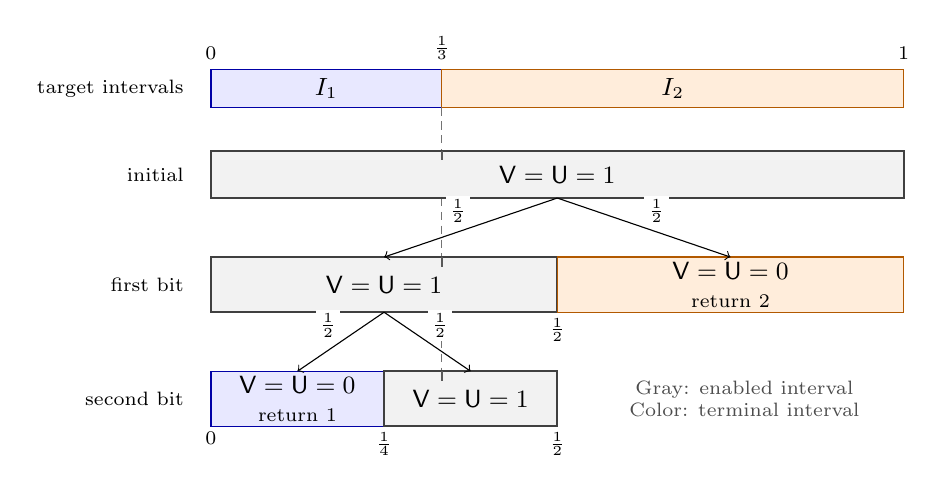
\begin{tikzpicture}[
   x=8.8cm,y=1cm,
   every node/.style={font=\small},
   active/.style={draw=black!75,fill=black!5,line width=.7pt},
   first/.style={draw=blue!65!black,fill=blue!9,line width=.5pt},
   second/.style={draw=orange!70!black,fill=orange!14,line width=.5pt},
   bit/.style={font=\scriptsize,fill=white,inner sep=1.5pt},
   rowlabel/.style={anchor=east,font=\scriptsize,align=right}
 ]
  % The target distribution, with its unique internal boundary.
  \path[first]  (0,0) rectangle (1/3,.48);
  \path[second] (1/3,0) rectangle (1,.48);
  \node at (1/6,.24) {$I_1$};
  \node at (2/3,.24) {$I_2$};
  \node[rowlabel] at (-.025,.24) {target\ intervals};
  \node[above,font=\scriptsize] at (0,.48) {$0$};
  \node[above,font=\scriptsize] at (1/3,.48) {$\tfrac13$};
  \node[above,font=\scriptsize] at (1,.48) {$1$};

  % Put the guide behind the arrows and their probability labels.
  \draw[densely dashed,black!55] (1/3,0) -- (1/3,-.55);
  \draw[densely dashed,black!55] (1/3,-1.15) -- (1/3,-1.90);
  \draw[densely dashed,black!55] (1/3,-2.60) -- (1/3,-3.35);

  % The initial interval J(0,1).
  \path[active] (0,-1.15) rectangle (1,-.55);
  \node at (.5,-.85) {$\mathsf V=\mathsf U=1$};
  \node[rowlabel] at (-.025,-.85) {initial};

  % First fair bit: left child continues, right child returns outcome 2.
  \path[active] (0,-2.60) rectangle (.5,-1.90);
  \path[second] (.5,-2.60) rectangle (1,-1.90);
  \node at (.25,-2.25) {$\mathsf V=\mathsf U=1$};
  \node[align=center] at (.75,-2.25)
    {$\mathsf V=\mathsf U=0$\\[-1pt]\scriptsize return $2$};
  \node[rowlabel] at (-.025,-2.25) {first\ bit};
  \draw[->] (.5,-1.15) -- node[bit,above left] {$\tfrac12$} (.25,-1.90);
  \draw[->] (.5,-1.15) -- node[bit,above right] {$\tfrac12$} (.75,-1.90);
  \node[below,font=\scriptsize,inner sep=2pt] at (.5,-2.60) {$\tfrac12$};

  % Refine only the still-enabled left child.
  \path[first]  (0,-4.05) rectangle (.25,-3.35);
  \path[active] (.25,-4.05) rectangle (.5,-3.35);
  \node[align=center] at (.125,-3.70)
    {$\mathsf V=\mathsf U=0$\\[-1pt]\scriptsize return $1$};
  \node at (.375,-3.70) {$\mathsf V=\mathsf U=1$};
  \node[rowlabel] at (-.025,-3.70) {second\ bit};
  \draw[->] (.25,-2.60) -- node[bit,above left] {$\tfrac12$} (.125,-3.35);
  \draw[->] (.25,-2.60) -- node[bit,above right] {$\tfrac12$} (.375,-3.35);
  \node[below,font=\scriptsize,inner sep=2pt] at (0,-4.05) {$0$};
  \node[below,font=\scriptsize,inner sep=2pt] at (.25,-4.05) {$\tfrac14$};
  \node[below,font=\scriptsize,inner sep=2pt] at (.5,-4.05) {$\tfrac12$};

  % Short boundary ticks at the top of each enabled interval.
  \draw[black!65,line width=.6pt] (1/3,-.55) -- (1/3,-.67);
  \draw[black!65,line width=.6pt] (1/3,-1.90) -- (1/3,-2.02);
  \draw[black!65,line width=.6pt] (1/3,-3.35) -- (1/3,-3.47);
  \node[align=center,font=\scriptsize,text=black!70] at (.77,-3.70)
    {Gray: enabled interval\\Color: terminal interval};
 \end{tikzpicture}
 \caption{Han--Hoshi for weights $(1,2)$.  Bars represent half-open
 intervals at their actual horizontal positions; the dashed guide marks
 the target boundary $1/3$.  A gray interval straddles this boundary and
 has $\mathsf V=\mathsf U=1$; a colored interval is contained in $I_1$ or
 $I_2$ and has value $0$.  Arrows show conditional probabilities for one
 complete loop iteration.  Only the enabled child is refined further.}
 \label{fig:han-hoshi-certificates}
\end{figure}


Interval-boundary counting thus supplies both certificates, complementing
the difference- and depth-based arguments for FDR and FLDR.
\Cref{app:han-hoshi-tail} derives a geometric tail bound from the same
one-iteration estimate.

\FloatBarrier
\section{Automatic Template-Based Certificate Synthesis}
\label{sec:certificate-synthesis}

We automatically search for AST certificates for probabilistic while
loops with loop-free bodies. Given a body encoding and an invariant,
our prototypical implementation constructs \emph{guarded affine}
or \emph{guarded piecewise affine} templates with integer coefficients
for the certificate functions $u$ and $v$.
The piecewise templates use a supplied finite partition.
Both classes assign zero when the loop guard is false.

The supported encodings use integer and Boolean state components.
Loop guards and conditional tests are Boolean combinations of linear
integer comparisons and Boolean flags. Right-hand sides of numerical
assignments are integer-valued piecewise affine expressions, whose
conditions use the same predicate fragment.
The supplied invariant and partition predicates also belong to this
fragment. The implementation accepts manually supplied Python/Z3
encodings of complete iterations; it does not parse source programs
or derive their semantics or invariants.

The search uses counterexample-guided inductive synthesis (CEGIS):
a learner proposes coefficients, and a verifier either validates them
over the entire invariant domain or returns a state that rules them out.
The random walk, FDR, and FLDR instantiate the same input interface and
algorithm, using exact or abstract descriptions of complete iterations.

\subsection{Loop Models, Templates, and Verification Conditions}
\label{sec:synthesis-constraints}

\paragraph{Supplied loop model.}
The input consists of integer and Boolean state components, a guard $b$,
an initial-state description, an invariant predicate $S$, and an encoding
of the possible outcomes of one complete body execution.
Initialization may be specified by an update; for FDR, this is
$(n,v,c)\mapsto(n,1,0)$ under $n\geq1$.

The predicates in the encoding are Boolean combinations of linear
integer comparisons and Boolean state components.
Integer components are updated by integer-valued piecewise affine
expressions: on each of finitely many regions defined by such
predicates, the update is affine.

We identify $S$ with the set of states satisfying it.
It is assumed to contain all initialized states and to be preserved
by every body outcome from an enabled state.
Thus, $S$ induces the distributional invariant
\[
 I=\{\mu\in\subdists\mid \operatorname{supp}(\mu)\subseteq S\}.
\]
This representation restricts the possible states in the support of
a distribution; it imposes no further constraints on their probabilities.

An exact body encoding specifies a finite number $h\geq1$ of
probabilistic outcomes, represented by update functions
$T_1,\ldots,T_h$ and fixed positive rational weights
$p_1,\ldots,p_h$ with $\sum_{j=1}^{h}p_j=1$.
Each $T_j$ maps the state before an iteration to its final state,
accounting for all assignments, tests, and choices, including any reset.
For every enabled state $\sigma\in S$, the encoding satisfies
\[
 \den{B}(\dirac{\sigma})
 =\sum_{j=1}^{h}p_j\,\dirac{T_j(\sigma)}.
\]
Different outcomes may yield the same final state.

The model is supplied as Python/Z3 expressions.
The implementation neither parses source programs nor derives
their semantics or invariants.

Read-only program parameters are state components that the updates leave
unchanged. For example, the FDR input $n$ remains unchanged during a run,
but can range over all positive integers in one synthesis problem.
These parameters are distinct from the unknown coefficients of a
certificate template. A fixed numerical input, such as the FLDR weights
$(4,5)$, is substituted into the model; an unspecified integer input
remains a symbolic state component.

\paragraph{Certificate templates.}
Let $x_1,\ldots,x_d$ be all declared integer components, including
symbolic read-only inputs, and write $x_i(\sigma)=\sigma(x_i)$ for
their values. The automatically constructed affine basis is
$(x_1,\ldots,x_d,1)$. Boolean flags may occur in the guard and in
partition predicates, but are not numerical basis elements.
For the supermartingale $v$ and variant $u$ of \Cref{thm:program-rule},
the single-region templates are
\[
 \begin{aligned}
 V_{\mathbf a}(\sigma)&=[b](\sigma)
   \left(a_0+\sum_{i=1}^{d}a_i x_i(\sigma)\right),\\
 U_{\mathbf u}(\sigma)&=[b](\sigma)
   \left(u_0+\sum_{i=1}^{d}u_i x_i(\sigma)\right).
 \end{aligned}
\]
Here $[b](\sigma)$ is $1$ when the loop is enabled and $0$ otherwise.
The integers in $\mathbf a=(a_0,\ldots,a_d)$ and
$\mathbf u=(u_0,\ldots,u_d)$ are the unknown template coefficients:
one coefficient vector defines a function for all states and all
admitted values of the symbolic inputs. The two vectors are independent
unknowns, although the constraints below couple the resulting functions.
We use $V,U$ for these program-level certificates in this section;
they instantiate $v,u$ and carry no control-location argument.

For example, the FDR variant template is
$[v<n](u_0+u_n n+u_v v+u_c c)$. The procedure searches for the
four coefficients; the program input $n$ remains universally quantified.
The active expression $n-v+c$ is obtained by setting
$(u_0,u_n,u_v,u_c)=(0,1,-1,1)$.

\paragraph{Verification conditions.}
For given $V,U$, require the following at every
$\sigma\models S\land b$:
\begin{gather}
 V(\sigma)\geq1,\qquad U(\sigma)\geq1,
 \label{eq:syn-positive}\\
 \sum_{j=1}^{h}p_j V(T_j(\sigma))\leq V(\sigma),
 \label{eq:syn-supermartingale}\\
 \bigvee_{j=1}^{h}\bigl(U(T_j(\sigma))\leq U(\sigma)-1\bigr),
 \label{eq:syn-progress}\\
 U(\sigma)\leq V(\sigma).
 \label{eq:syn-domination}
\end{gather}
These conditions impose positivity, the supermartingale inequality,
probabilistic decrease, and sublevel boundedness, respectively.
A decreasing outcome has probability at least $\varepsilon=\min_jp_j>0$,
computed from the supplied weights. Since $U$ is integer-valued,
$U\leq V$ implies $U\leq\lfloor r\rfloor$ whenever $V\leq r$.
Every experiment below has two fair-bit outcomes, denoted $T_0,T_1$.
There the expectation condition becomes
$V(T_0(\sigma))+V(T_1(\sigma))\leq2V(\sigma)$ and
$\varepsilon=1/2$.
Requiring $U\leq V$ and integer-coefficient templates restricts the
search beyond the general rule, which permits real-valued
supermartingales and more general sublevel bounds.

\begin{proposition}[Soundness of the synthesis constraints]
\label{prop:synthesis-soundness}
Suppose $S$ contains the initial loop-head states and is preserved by
every outcome of an exact body encoding from enabled states.
Every template instantiation
satisfying \eqref{eq:syn-positive}--\eqref{eq:syn-domination} supplies
certificates for \Cref{thm:program-rule} with
$\varepsilon=\min_jp_j$.
\end{proposition}
\begin{proof}
Take $I=\{\mu\in\subdists\mid\supp(\mu)\subseteq S\}$, which is
a distributional invariant by the assumptions on $S$.
The guarded templates vanish on terminal states; on enabled states,
$V$ is positive and $U$ is a positive integer. The weighted inequality
is the required expectation bound. At least one outcome of weight
at least $\min_jp_j$ decreases $U$, and $U\leq V$ bounds $U$ by
$\lfloor r\rfloor$ on each $V$-sublevel. Thus all premises hold.
\end{proof}

\paragraph{Supplied abstractions of the body.}
The synthesis model need not represent a data structure used by the
loop body explicitly. For FLDR, an abstract model records whether
each fair-bit outcome continues, resets, or accepts, without encoding
the full sampling tree. It retains structural restrictions, such as
the fact that the two outcomes cannot both reset. Each bit outcome
still has probability $1/2$.

More generally, auxiliary variables $\xi$ describe possible successor
updates, and $A(\sigma,\xi)$ specifies their permitted combinations.
For each enabled state $\sigma\in S$ and each $\xi$ satisfying
$A(\sigma,\xi)$, the updates and their fixed probabilities define
the successor distribution
\[
 \sum_{j=1}^{h}p_j\cdot\dirac{T_j(\sigma,\xi)}.
\]
The verifier checks the certificate conditions for every such
distribution.

To establish AST of the concrete program, every concrete successor
distribution, expressed in the model's state variables, must belong
to this family. This inclusion must be justified separately;
for FLDR, it follows from the sampling-tree properties established
in Appendix~\ref{app:calculations}.
The automated checks below ensure that every enabled state admits
at least one description and that all represented outcomes preserve
the invariant.

\subsection{Counterexample-Guided Search and Fixed Partitions}
\label{sec:synthesis-cegis}

Before synthesis, the implementation checks that the supplied invariant
contains the initialized states and is preserved by every represented
outcome. An abstract model must also admit at least one successor
description at every enabled state.

For a fixed integer coefficient bound, the CEGIS learner proposes
coefficients satisfying \eqref{eq:syn-positive}--\eqref{eq:syn-domination}
on a finite set of samples. The verifier then searches the entire
invariant domain for a violating state, together with an admissible
transition description for abstract models. A counterexample extends the
sample set; an unsatisfiable query validates the pair universally.
The implementation accepts it only after rechecking each condition
separately. The coefficient bound restricts the candidate expressions,
not the states or symbolic program inputs over which they are verified.

\paragraph{Supplied partitions.}
\label{sec:synthesis-piecewise}
For piecewise affine certificates, the caller supplies a finite partition
of the enabled states. The implementation checks coverage and disjointness
and creates separate affine coefficient blocks for each region and
certificate. At a successor state, the applicable region is evaluated
again, so transitions between regions are checked as well.
Only the coefficients are synthesized; the partition predicates are fixed.

\Cref{app:synthesis-search} gives the search algorithm, coefficient
schedule, and template construction. Resource limits and unknown solver
answers are inconclusive. An unsuccessful search does not refute AST:
the finite coefficient schedule, templates, domination condition, and
supplied invariant restrict the search beyond
\Cref{thm:program-rule}.

\subsection{Instantiations and Experimental Results}
\label{sec:synthesis-examples}

\Cref{tab:synthesis-results} reports the automatically synthesized
certificates for five loop models. All coefficients were found by the
same engine from the supplied models and, in the last row, a supplied
partition. Each pair was verified over its entire invariant domain;
symbolic inputs were not restricted to finitely many numerical values.
The recorded run uses Z3~4.15.4 with ten seconds per solver call.
Detailed encodings and certificate analyses are in
\Cref{app:synthesis-models}; commands, logs, and additional checks are
described in \Cref{app:synthesis-checks}.

\begin{table}[t]
\centering\small
\setlength{\tabcolsep}{4pt}
\begin{tabular}{@{}llllr@{}}
\toprule
Loop model & $V$ & $U$ & $B$ & Candidates\\
\midrule
Random walk & $x$ & $x$ & 1 & 2\\
FDR, symbolic $n$ & $n$ & $n-v+c$ & 1 & 3\\
FLDR, weights $(4,5)$ & $c-2d+2$ & $c-2d+2$ & 2 & 4\\
FLDR, abstract family & $m$ & $k-c$ & 1 & 3\\
Two-sided walk, supplied split & $|x|$ & $|x|$ & 1 & 3\\
\bottomrule
\end{tabular}
\caption{Synthesized expressions on active states, with terminal values zero.
$B$ is the successful coefficient bound; candidate counts include earlier
bounds. The exact and abstract loop models are specified in
\Cref{app:synthesis-models}.}
\label{tab:synthesis-results}
\end{table}

\paragraph{Affine certificates.}
For the unbounded random walk, synthesis recovers $V=U=x$ from
\Cref{sec:rule-examples}. For FDR, it recovers $V=n$ and $U=n-v+c$
from \Cref{thm:fdr}, uniformly for all positive integer inputs $n$.
For the exact FLDR tree with weights $(4,5)$, the synthesized function
$c-2d+2$ serves as both certificates. Its expected value at the root
is unchanged after one iteration, illustrating that the constraints
do not require a uniformly negative expected drift.

\paragraph{FLDR with symbolic inputs.}
The abstract FLDR model represents arbitrary weight vectors through the
structural properties of their sampling trees. It retains the total
weight $m$, height bound $k$, and depth $c$ as symbolic components;
synthesis finds the pair $V=m$, $U=k-c$. The depth variant can increase in
expectation because of possible resets, while the separate supermartingale satisfies
the expectation bound. Verification covers every transition admitted
by the abstraction; its connection to concrete FLDR follows from the
tree argument in \Cref{app:calculations}. The fixed-tree result above
shows that distinct functions are not intrinsically necessary.

\paragraph{The benefit of a supplied partition.}
For the symmetric walk on all of $\mathbb Z$, terminating at $0$, the
split $x<0$ versus $x\geq0$ yields $V=U=|x|$. No single affine variant
can be both positive on the two unbounded tails and satisfy progress,
regardless of its coefficient bound
(\Cref{app:synthesis-models}). Thus the partition makes a certificate
expressible that a single affine template cannot represent.

These experiments demonstrate automatic coefficient search and universal
verification for supplied loop models. Semantics, invariants, abstraction
arguments, and partitions remain inputs. We do not compare performance
with existing tools.

\section{Related Work}
\label{sec:relwork}

\paragraph{AST proof rules.}
Bounded variants establish AST through a uniformly positive probability
of descent in a bounded natural-valued range~\cite{DBLP:series/mcs/McIverM05}.
McIver et al.~\cite{10.1145/3158121} give a source-level rule, including
demonic choice, in which a single real-valued function satisfies both
supermartingale and probabilistic progress obligations. Majumdar and
Sathiyanarayana~\cite{DBLP:journals/pacmpl/MajumdarS25} separate these roles
at pCFG level and prove relative completeness in arithmetic, also
establishing completeness of the earlier single-function rule.
Our contribution concerns the representation of certificates and their
transfer to whole iterations, rather than greater semantic proving power.
Separating the roles allows a resetting variant without requiring that
particular variant to be a supermartingale; it does not show that every
single-function certificate must fail.

\paragraph{Distribution transformers and program logics.}
Kozen's semantics~\cite{DBLP:conf/focs/Kozen79,DBLP:conf/stoc/Kozen83}
provides the denotational foundation for our post-distribution
transformers. Expectation-transformer reasoning~\cite{DBLP:series/mcs/McIverM05}
and distributional program logics, including den Hartog and de
Vink~\cite{DBLP:journals/ijfcs/HartogV02} and
Ellora~\cite{DBLP:conf/esop/BartheEGGHS18}, support broader probabilistic
correctness properties. Our AST rule complements such reasoning:
distributional invariants can carry output information, while termination
uses their support and two state functions. Thus, the rule does not
replace distributional output-correctness arguments.

\paragraph{Certificate and invariant synthesis.}
Constraint-based methods synthesize martingale and ranking-supermartingale
certificates~\cite{ChakarovSankaranarayanan2013}. Batz et
al.~\cite{BatzEtAl2023} synthesize piecewise linear quantitative invariants
that certify bounds on expected outcomes and finite expected runtime.
Their counterexample-guided approach operates at source level and also
supports infinite-state programs.
We instantiate this search pattern with two AST certificates and the
sufficient coupling $U\leq V$. The random
walk illustrates qualitative termination with infinite expected runtime.
Neither CEGIS nor affine or piecewise affine templates are new here.
The contribution is their explicit instantiation for these two
iteration-level certificate roles. State components, invariants, transition summaries, and partitions
remain supplied inputs; the affine basis is generated from all declared
integer components and the constant term. Bounded search is incomplete
even though successful candidates are checked universally over the
encoded states.

Haase et al.~\cite{haase2026generatingfunctionsmeetoccupation} generalize
probability generating functions to occupation measures and synthesize
occupation invariants in this representation. The coefficients bound
expected visit counts and need not sum to one.
These invariants support exact inference,
with positive AST obtainable under suitable finiteness conditions.
Their unknowns and verification conditions therefore differ from our
state-function certificates for qualitative AST. Template instantiation
is common to both approaches, but their results are not interchangeable.

\paragraph{Exact samplers and their verification.}
The algorithms studied here are established constructions:
Lumbroso's FDR~\cite{DBLP:journals/corr/abs-1304-1916}, Saad et al.'s
FLDR~\cite{DBLP:conf/aistats/SaadFRM20}, and Han and Hoshi's interval
algorithm~\cite{HanHoshi1997}. Zilken et
al.~\cite{zilken2026verifyingsamplingalgorithmsdistributional}
verify partial and total correctness of FDR and FLDR, combining
distributional invariants with the pCFG two-certificate AST rule.
The present paper formulates and proves a general iteration-level rule,
then revisits these AST arguments through that interface. We make the
required support assertions explicit; for FLDR, we establish the
valid-node assertion for the tree convention used here.
Han--Hoshi supplies a different termination argument, rather than
a new output-correctness proof.
Bagnall et al.'s Zar compiler~\cite{DBLP:journals/pacmpl/Bagnall0023}
verifies compilation of probabilistic programs into random-bit samplers
in Coq. Our handwritten proofs and solver-backed prototype do not
provide that level of mechanization.

\paragraph{Nondeterminism.}
The rules of McIver et al.~\cite{10.1145/3158121} and Majumdar and
Sathiyanarayana~\cite{DBLP:journals/pacmpl/MajumdarS25} support
demonic nondeterminism. Our current
transformer assigns one post-distribution to each input. Extending the
rule to universal scheduler quantification requires corresponding
semantic and progress obligations. Programmatic strategy
synthesis~\cite{DBLP:journals/pacmpl/BatzBKW24} instead resolves
nondeterminism to obtain a selected program; it addresses a different
quantification over choices.

\section{Conclusion}
\label{sec:conclusion}

We presented a sound and relatively complete program-level AST rule for
fixed-probability loops with loop-free bodies. Users supply two state
functions at loop heads; the certificate translations account for internal
control locations. The rule uses distributional-invariant support, leaving
quantitative output information available.

The sampler proofs cover recycling, restart, and interval refinement.
They illustrate the proof interface without establishing that distinct
certificates are necessary. The unbounded random walk demonstrates AST
with infinite expected runtime.

A bounded CEGIS kernel synthesizes guarded affine and fixed-partition
piecewise affine certificates. Successful candidates are checked over
the full supplied invariant domains. Invariants, iteration semantics,
partitions, and abstraction arguments remain inputs, while $U\leq V$
restricts the coupling. Relative completeness of the rule therefore does
not transfer to the search. Richer templates and automatic input generation
remain future work.

Nested loops require AST summaries and a new compositional argument:
unbounded inner executions invalidate the bounded-path translation.
For nondeterministic programs, \emph{demonic} semantics requires AST
under every scheduler resolving the choices. An extension would therefore
need invariant preservation and supermartingale inequalities for all
admissible body distributions, together with a uniform variant-progress
guarantee. Checking one selected distribution covers only that behavior;
soundness of the extension remains to be established.


\paragraph{Data availability.}
The accompanying package \texttt{AST\_Synthesis\_Artifact.zip} contains the
synthesis implementation, input encodings, pinned dependency, recorded
results, and exact-arithmetic diagnostics. Its README gives reproduction
commands and maps outputs to the paper. No externally collected dataset
is used. The metatheory is not mechanized; the implementation checks the
supplied synthesis obligations.

\bibliographystyle{splncs04}
\bibliography{references}

\ifappendixversion
\clearpage
\appendix
\section{Translation and AST Preservation}
\label[appendix]{app:translation}

\paragraph{Well-defined loop semantics.}
The transformer domain $\mathcal{H}$ from \Cref{sec:prelims} has pointwise suprema of increasing $\omega$-chains: these preserve $\omega$-continuity and the mass bound by monotone convergence. Its least element is $\bot=\lambda\eta.0$. By structural induction, the body transformer $\post{B}$ is $\omega$-continuous and does not increase mass. For $f\in\mathcal{H}$ and $\eta\in\subdists$,
\[
 \weight{\Phi_{b,B}(f)(\eta)}
 =\weight{[\neg b]\eta}
   +\weight{f\bigl(\post{B}([b]\eta)\bigr)}
 \leq\weight{[\neg b]\eta}+\weight{[b]\eta}
 =\weight{\eta}.
\]
Composition and addition preserve $\omega$-continuity here, so $\Phi_{b,B}(f)\in\mathcal{H}$. Moreover, for every increasing chain $(f_n)_n$ in $\mathcal{H}$, pointwise evaluation gives $\Phi_{b,B}(\sup_n f_n)=\sup_n\Phi_{b,B}(f_n)$. Kleene's theorem therefore yields \Cref{eq:while-transformer-fixpoint}. Structural induction also establishes linearity on sums that are subdistributions: in the loop case, every approximant is linear, and its pointwise supremum remains linear. The countable-sum property follows from $\omega$-continuity.

\paragraph{Operational correspondence.}
We use the pCFG notation of \Cref{sec:pcfg-rule}.
The translation $\mathcal{T}$ assigns distinct entry and exit locations to each command, with fresh internal locations for its subcommands. Skip is a single identity edge. Assignments are single update edges. A conditional entry has guarded edges to the two branch entries; a probabilistic-choice entry instead has edges of probabilities $p$ and $1-p$. In either case the branch exits are identified with the command exit. Sequential composition identifies the first command's exit with the second command's entry. For a while-loop, its entry is the guard: the true edge enters the body, the false edge reaches the program exit, and the body exit is identified with the guard. Zero-probability edges are ignored, and the program exit is absorbing. Thus the loop-free body is acyclic and every path through it contains at least one edge.

For the isolated body graph $\mathcal T[B]$, let $\ell_{\rm in}$ and
$\ell_{\rm out}$ be its entry and exit; the latter becomes the guard
when the body is embedded in the loop. Write
$\mathcal P_B(\sigma,\sigma')$ for the finite set of positive-probability
configuration paths from $(\ell_{\rm in},\sigma)$ to their first visit
to $(\ell_{\rm out},\sigma')$. For a path
$\pi=(\gamma_0,\ldots,\gamma_n)$, put
$w(\pi)=\prod_{i=0}^{n-1}P(\gamma_i,\gamma_{i+1})$.

\begin{lemma}[Loop-free correspondence]
For loop-free $B$ and states $\sigma,\sigma'$,
\[
 \post{B}(\dirac{\sigma})(\sigma')
 =\sum_{\pi\in\mathcal P_B(\sigma,\sigma')}w(\pi).
\]
\end{lemma}
\begin{proof}
By structural induction on $B$. Skip and assignment have one path. Sequential composition sums over intermediate states. Conditional paths are partitioned by the guard. Probabilistic choice multiplies branch-path probabilities by $p$ and $1-p$, matching linearity of the distribution transformer.
\end{proof}

For a loop $C=\while{b}{B}$ with loop-free body, induction on $j$ shows that $\Phi_{b,B}^{j}(\bot)(\mu)$ is the subdistribution of pCFG runs that exit within at most $j$ visits to the outer loop guard. The zeroth approximant is zero; for $j\geq1$, this means termination after at most $j-1$ completed body iterations. The induction step partitions runs into those that exit at the first guard test and those that execute $B$ and then terminate within the remaining guard visits. Taking pointwise suprema gives equality between post-distribution weight and pCFG reachability probability. Therefore $\weight{\post{C}(\dirac{\sigma})}=1$ iff the translated graph reaches its exit almost surely from the loop guard with valuation $\sigma$. For any initial subdistribution,
\[
 \weight{\mu}-\weight{\post{C}(\mu)}
 =\sum_{\sigma\in\supp(\mu)}\mu(\sigma)
     \bigl(1-\weight{\post{C}(\dirac{\sigma})}\bigr).
\]
Every summand is nonnegative, so the left-hand side vanishes exactly when
$C$ is AST from every state in $\supp(\mu)$. Taking the union over
$\mu\in M$ proves the AST-preservation equivalence \eqref{eq:ast-preservation}
for arbitrary $M$.

\subsection{Common Certificates for Initial-State Sets}
\label[appendix]{app:initial-sets}

The pCFG completeness construction
of~\cite{DBLP:journals/pacmpl/MajumdarS25} is presented for a fixed initial
configuration. We record why it also supplies a single pair of
certificates for the initial-state sets used here. We use the purely probabilistic model with fixed rational probabilities.
Computability of the operations is needed only for the arithmetic
representation below.

Let $E$ be any set of initial valuations from which the pCFG is AST, and
let $\mathit{Inv}$ contain exactly the configurations reachable from $E$
by positive-probability paths. Every configuration in $\mathit{Inv}$ is
AST: otherwise, a positive-probability path to a configuration with
positive divergence probability would give positive divergence probability
from an initial state. Set $U(\gamma)$ to the length of a shortest
positive-probability path from $\gamma$ to the program exit. Such a finite
path exists by AST. Hence $U$ is zero exactly at the exit and strictly
decreases at the unique successor of a deterministic nonterminal
configuration and at some successor of a probabilistic configuration.
The minimum of $1$ and the positive probabilistic edge probabilities
of the finite pCFG gives a common positive progress bound.

It remains to construct a compatible $V$. Fix an injective encoding
$\operatorname{code}:L\times\Sigma\hookrightarrow\mathbb N$,
computable for finite rational state tuples. Let $(\Gamma_t)_{t\in\mathbb N}$
be the Markov chain with transition probabilities $P$, and let
$\Pr\nolimits_\gamma$ denote its law when started at $\gamma$.
Its first exit time is
$T=\inf\{t\in\mathbb N\mid\Gamma_t\text{ is terminal}\}$,
with $\inf\varnothing=\infty$. For $\gamma\in\mathit{Inv}$ and
$n\in\mathbb N$, define
\[
 R(\gamma,n)=\Pr\nolimits_\gamma
 \bigl(\exists t<T:\ \operatorname{code}(\Gamma_t)\geq n\bigr).
\]
This event includes the starting configuration when it is nonterminal;
for terminal $\gamma$ its probability is zero.
For fixed $n$, this function is a nonnegative supermartingale: outside
the target set the first-step equation is an equality, and in the target
set its value is $1$. Moreover,
\[
 \lim_{n\to\infty}R(\gamma,n)=0.
\]
Indeed, an almost-surely terminating run visits only finitely many
configurations before its first exit, so the corresponding decreasing
tail events have an intersection of probability zero.

For every $k\geq1$, choose the least integer $n_k\geq k$ such that
\[
 R(\gamma,n_k)\leq2^{-k}
 \quad\text{for all }\gamma\in\mathit{Inv}
                     \text{ with }\operatorname{code}(\gamma)\leq k.
\]
Only finitely many configurations are constrained for each $k$, so this
integer exists. Define
\[
 V(\gamma)=[\gamma\text{ is nonterminal}]
              +\sum_{k=1}^{\infty}R(\gamma,n_k).
\]
For a fixed configuration with code $i$, the summands with $k\geq\max(1,i)$
are bounded by $2^{-k}$; thus $V$ is finite everywhere. The indicator
is itself a supermartingale because the exit is absorbing. Nonnegative
summation preserves the supermartingale inequalities, and the indicator
term makes $V$ positive at every nonterminal configuration and zero at
the exit. Given $r\geq0$, choose an integer $m>r$. Any nonterminal
configuration with code at least $\max\{n_1,\ldots,n_m\}$ belongs to all
first $m$ target sets, and hence has $V\geq1+m>r$. Consequently,
$V_{\leq r}$ contains only finitely many nonterminal configurations.
As $U=0$ at terminal configurations, $U$ is bounded on every sublevel
set. This proves semantic completeness for arbitrary $E$, including
infinite sets, without any uniform bound on initial certificate values.
The empty initial set is handled by the empty invariant.

\paragraph{Arithmetic representation.}
If $E$ is arithmetically definable, so is $\mathit{Inv}$: quantify over
an initial state in $E$ and an encoded finite feasible path. The same
encoding defines the graph of the shortest-path function $U$. For a finite horizon $t$, let $h_t(\gamma,n)$ be the probability of
hitting a nonterminal configuration of code at least $n$ by step $t$
before termination. It is a computable rational number, uniformly in
its arguments, because the transition tree to depth $t$ is finite.
Since $R(\gamma,n)=\sup_t h_t(\gamma,n)$, for rational $q$,
\begin{align*}
 q<R(\gamma,n)&\ \Longleftrightarrow\ \exists t:\ q<h_t(\gamma,n),\\
 R(\gamma,n)\leq q&\ \Longleftrightarrow\ \forall t:\ h_t(\gamma,n)\leq q.
\end{align*}
Thus the defining property and minimality of $n_k$ give an arithmetic
graph for the sequence, using the arithmetic predicate for
$\mathit{Inv}$. To encode the strict lower cut of $V$, write
$d_\gamma=[\gamma\text{ is nonterminal}]$. Then $q<V(\gamma)$ iff
there exist $m\in\mathbb N$ and an encoded rational sequence
$(q_1,\ldots,q_m)$ such that
\[
 q<d_\gamma+\sum_{k=1}^m q_k
 \quad\text{and}\quad
 q_k<R(\gamma,n_k)\text{ for every }1\leq k\leq m.
\]
The empty sequence is allowed. This equivalence follows from convergence
of the nonnegative series and density of the rationals for each finite
partial sum. It supplies one arithmetic formula, rather than a separate
formula for each bound or configuration. No effective enumeration of
$E$, and no computation of the infinite sum, is required. These are
expressibility statements relative to true arithmetic.

\paragraph{Encoding the verification conditions.}
\label{app:arithmetic-obligations}
Let $f_1,\ldots,f_d,g$ be finite real-valued functions with arithmetic
strict lower cuts $\theta_{f_i}(\sigma,q)$ and $\theta_g(\sigma,q)$,
and let $p_1,\ldots,p_d$ be positive rational constants. A strict lower
cut for their weighted sum is
\[
 \begin{aligned}
 q<\sum_{i=1}^d p_i f_i(\sigma)
 \quad\Longleftrightarrow\quad
 &\exists q_1,\ldots,q_d\in\mathbb Q:\\
 &q<\sum_{i=1}^d p_iq_i\ \land\
 \bigwedge_{i=1}^d\theta_{f_i}(\sigma,q_i).
 \end{aligned}
\]
For any two such functions $f,g$, cut inclusion expresses comparison:
\[
 f(\sigma)\leq g(\sigma)
 \ \Longleftrightarrow\
 \forall q\in\mathbb Q:
 \quad\theta_f(\sigma,q)\Longrightarrow\theta_g(\sigma,q).
\]
Both equivalences follow from density of the rationals. Composing these
formulas with the computable updates of each feasible body path gives
the expected-value obligation. Feasibility predicates select the relevant
paths from a fixed finite list. Variant comparisons use the arithmetic
graph of $u$, so the progress probability is a finite rational sum
selected by arithmetic conditions. Sublevel boundedness quantifies over
natural thresholds and bounds; $v(\sigma)\leq r$ is represented by
$\neg\theta_v(\sigma,r)$. Thus all certificate obligations are first-order
arithmetic sentences, although the certificate values need not be rational.

\section{Detailed One-Iteration Calculations}
\label[appendix]{app:calculations}

\subsection{FDR: Complete Updates and Support Preservation}
Starting from an enabled state with integer $n,v,c$,
$1\leq v<n$ and $0\leq c<v$, a bit $\beta$ gives
$t=2c+\beta$ and $0\leq t<2v<2n$.
If $t<n$, the complete successor is $(2v,t)$ and satisfies
$0\leq t<\min(2v,n)$. If $t\geq n$, the successor is
$(2v-n,t-n)$; here $1\leq2v-n<n$ and
$0\leq t-n<2v-n$. Both cases preserve \eqref{eq:fdr-support}, and
initialization gives $(v,c)=(1,0)$ for every $n\geq1$.
The probability-weighted sum of these complete updates is exactly
\eqref{eq:fdr-post}. In both cases the updated difference is
\[
 v'-c'=2(v-c)-\beta.
\]
For $\beta=0$, a continuing outcome satisfies
\[
 n-v'+c'=n-v+c-(v-c)\leq n-v+c-1.
\]
A terminal outcome has guarded certificate zero. This proves the
affine descent used in \Cref{thm:fdr} over the entire supplied support,
not merely the states reachable for one fixed $n$.
The same difference identity also gives the logarithmic descent for
\eqref{eq:fdr-log-variant}.

\subsection{FDR: Shortest Paths and a Logarithmic Variant}
\label[appendix]{app:fdr-log-variant}
The logarithmic variant used in the earlier FDR AST argument
\cite{zilken2026verifyingsamplingalgorithmsdistributional} also fits
the present rule. Keeping $I_{\mathrm{FDR}}$, $v$, and
$\varepsilon=1/2$ fixed, we may choose
\begin{equation}
 u_{\log}(\sigma)=
 \begin{cases}
 \left\lceil\log_2\!\left(\dfrac{n}{v-c}\right)\right\rceil,&v<n,\\
 0,&v\geq n.
 \end{cases}
 \label{eq:fdr-log-variant}
\end{equation}
For an enabled state, $1\leq v-c<n$, so the logarithm is positive
and finite; the ceiling makes $u_{\log}$ a positive integer.
This variant is motivated by the number of complete iterations needed
to reach a terminal state along a possible sequence of bits.
Write $d_{\min}(\sigma)$ for the shortest such number: a step from
an enabled state is one complete update $F_0$ or $F_1$, and the target
is any state with $v\geq n$. Terminal states have distance zero.

To see that a finite path to termination exists, put $\Delta=v-c$.
Every zero-bit iteration doubles $\Delta$, including iterations that
recycle. After
$k=\lceil\log_2(n/\Delta)\rceil$ consecutive zero bits, either the loop
has terminated or its difference would be $2^k\Delta\geq n$.
The latter is impossible at an enabled loop head, where
$\Delta\leq n-1$. This sequence therefore reaches a terminal state
within $k$ iterations and has probability at least $2^{-k}>0$. Hence
\begin{equation}
 d_{\min}(\sigma)\leq u_{\log}(\sigma).
 \label{eq:fdr-shortest-distance-bound}
\end{equation}
The bound need not be exact. For $n=6$ and $(v,c)=(4,2)$, it gives
$u_{\log}=2$, but both successors $(8,4)$ and $(8,5)$ are terminal,
so $d_{\min}=1$. \Cref{fig:fdr-iteration-variants} compares the
logarithmic variant $u_{\log}$ with the exact distance $d_{\min}$.

The zero-bit outcome proves descent of $u_{\log}$ directly: if it
continues, then
\[
 u_{\log}(F_0(\sigma))
 =\left\lceil\log_2\!\left(\frac{n}{2(v-c)}\right)\right\rceil
 =u_{\log}(\sigma)-1;
\]
if it terminates, its value is zero. On enabled states with
$v(\sigma)\leq r$, we have $n\leq r$ and therefore
$u_{\log}\leq\lceil\log_2 n\rceil\leq\lceil\log_2 r\rceil$.
For $r<1$, the sublevel contains only terminal states.
Thus $u_{\log}$ satisfies the same rule.
The distance $d_{\min}$ is another valid variant: the first bit of
a shortest path decreases it by one with probability at least $1/2$,
and \eqref{eq:fdr-shortest-distance-bound} supplies its sublevel bound.
The affine variant avoids both a logarithm and a shortest-path
calculation, which is why we use it for the main proof.

% This new drawing contracts all recycling updates and shows actual
% shortest distances alongside the terminal-normalized logarithmic variant.
\begin{figure}[t]
 \centering
 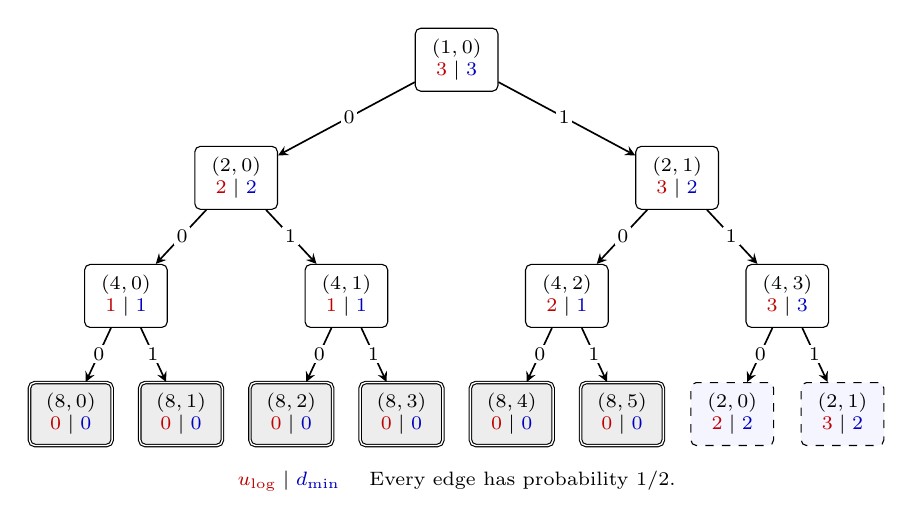
\begin{tikzpicture}[
   x=1.4cm,y=1cm,>=stealth,
   fdrstate/.style={draw,rounded corners=2pt,minimum width=10.5mm,
     minimum height=8mm,inner sep=2pt,align=center,font=\scriptsize},
   fdrterminal/.style={fdrstate,fill=black!7,double,double distance=0.5pt},
   fdrrecycled/.style={fdrstate,dashed,fill=blue!4},
   fdrbit/.style={font=\scriptsize,fill=white,inner sep=1pt},
   fdredge/.style={->,semithick}
 ]
 % Each node displays (v,c), then u_log | d_min.
 \node[fdrstate] (s10) at (3.5,4.5)
   {$(1,0)$\\$\textcolor{red!75!black}{3}\mid\textcolor{blue!75!black}{3}$};
 \node[fdrstate] (s20) at (1.5,3)
   {$(2,0)$\\$\textcolor{red!75!black}{2}\mid\textcolor{blue!75!black}{2}$};
 \node[fdrstate] (s21) at (5.5,3)
   {$(2,1)$\\$\textcolor{red!75!black}{3}\mid\textcolor{blue!75!black}{2}$};
 \node[fdrstate] (s40) at (0.5,1.5)
   {$(4,0)$\\$\textcolor{red!75!black}{1}\mid\textcolor{blue!75!black}{1}$};
 \node[fdrstate] (s41) at (2.5,1.5)
   {$(4,1)$\\$\textcolor{red!75!black}{1}\mid\textcolor{blue!75!black}{1}$};
 \node[fdrstate] (s42) at (4.5,1.5)
   {$(4,2)$\\$\textcolor{red!75!black}{2}\mid\textcolor{blue!75!black}{1}$};
 \node[fdrstate] (s43) at (6.5,1.5)
   {$(4,3)$\\$\textcolor{red!75!black}{3}\mid\textcolor{blue!75!black}{3}$};
 \foreach \j in {0,...,5} {
   \node[fdrterminal] (t\j) at (\j,0)
     {$(8,\j)$\\$\textcolor{red!75!black}{0}\mid\textcolor{blue!75!black}{0}$};
 }
 \node[fdrrecycled] (r20) at (6,0)
   {$(2,0)$\\$\textcolor{red!75!black}{2}\mid\textcolor{blue!75!black}{2}$};
 \node[fdrrecycled] (r21) at (7,0)
   {$(2,1)$\\$\textcolor{red!75!black}{3}\mid\textcolor{blue!75!black}{2}$};
 \foreach \from/\to/\bit in {
   s10/s20/0,s10/s21/1,
   s20/s40/0,s20/s41/1,s21/s42/0,s21/s43/1,
   s40/t0/0,s40/t1/1,s41/t2/0,s41/t3/1,
   s42/t4/0,s42/t5/1,s43/r20/0,s43/r21/1} {
   \draw[fdredge] (\from) -- node[fdrbit,pos=0.48] {$\bit$} (\to);
 }
 \node[font=\scriptsize,align=center] at (3.5,-0.85)
   {$\textcolor{red!75!black}{u_{\log}}\mid\textcolor{blue!75!black}{d_{\min}}$
    \quad Every edge has probability $1/2$.};
 \end{tikzpicture}
 \caption{Three-iteration unfolding of FDR for $n=6$. Each node gives
 $(v,c)$ and, below it, the logarithmic variant $u_{\log}$ (red, left) and the
 shortest distance $d_{\min}$ (blue, right). Edge labels are sampled bits.
 Double borders mark terminal states, where both functions are zero.
 Dashed leaves repeat earlier states after recycling; they are not
 terminal. Each edge includes all updates of one loop iteration.}
 \label{fig:fdr-iteration-variants}
\end{figure}

\subsection{FLDR: The Exact Tree Contract}
Put $w_i=a_i$ for $1\leq i\leq n$ and $w_{n+1}=2^k-m$, so
$\sum_iw_i=2^k$. For $0\leq c\leq k$, let $e_{i,c}\in\{0,1\}$ be
the bit of $w_i$ in position $k-c$, and put $h_c=\sum_i e_{i,c}$.
At depth zero there is one node. Designate $h_0$ nodes as leaves and
put $q_0=1-h_0$. At each subsequent depth $c$, expand the $q_{c-1}$
internal nodes, producing $2q_{c-1}$ nodes, and designate $h_c$ of
them as leaves. Thus
\[
 q_c=2q_{c-1}-h_c
     =2^c-\sum_{i=1}^{n+1}
         \left\lfloor\frac{w_i}{2^{k-c}}\right\rfloor
     =\sum_{i=1}^{n+1}
         \left\{\frac{w_i}{2^{k-c}}\right\},
\]
where braces denote fractional part. Consequently $q_c$ is a
nonnegative integer at most $n$, and $q_k=0$. In particular, the
construction always has enough nodes for its designated leaves and
has no internal node at depth $k$.

Set $\phi_h(c)=q_c$. In every row place the internal nodes first and
then one leaf labeled $i$ for each $e_{i,c}=1$, in decreasing label
order. At positive depth the row has $2q_{c-1}\leq2n$ nodes.
An internal node with index $d<q_c$ therefore has the two valid children
$2d,2d+1$ in the next row. Give internal nodes label zero in $H$.
A root leaf occurs precisely when a single positive weight equals
$2^k$; it is accepting, since $w_{n+1}<2^k$.
These observations justify the support predicate in
\Cref{sec:fldr}, including $d<2n$ and the absence of enabled states at
depth $k$. A tighter bound $d\leq n$ would be false: for weights
$(4,5)$, the accepting node $(c,d)=(2,3)$ is reachable although $n=2$.

Each row has at most one leaf with label $n+1$. Hence among the two
children of any internal node at least one avoids rejection. A rejecting
child resets to the root, which is internal whenever a rejecting leaf
exists. A non-rejecting child either accepts or remains internal at
depth $c+1$. Thus the post-distribution has non-reset mass at least
$1/2$, and every such outcome strictly decreases the guarded function
$k-c$. This is the structural contract used by the abstract synthesis
instance. It follows from the construction for all positive integer
weight vectors; finite checks of generated trees are additional tests,
not a replacement for this argument.

For completeness, the leaf construction also preserves the proposal
probabilities. A leaf labeled $i$ at depth $c$ has probability $2^{-c}$,
so one traversal returns $i$ with probability
$\sum_c e_{i,c}2^{-c}=w_i/2^k$. Rejection restarts from the root.
Writing $p_i$ for the eventual probability of outcome $i$, first-traversal
conditioning gives
\[
 p_i=\frac{a_i}{2^k}+\frac{2^k-m}{2^k}p_i,
 \qquad\text{hence}\qquad p_i=\frac{a_i}{m}.
\]
The AST proof ensures that these probabilities account for the entire
output mass. This direct argument also confirms that reordering leaves
within a row does not alter the sampled distribution.

\subsection{Han--Hoshi: Boundary Counting and a Tail Bound}
\label[appendix]{app:han-hoshi-tail}
For a nonempty interval $J\subseteq[0,1)$, containment in a target
interval is equivalent to having no internal target boundary strictly
inside $J$. An endpoint coinciding with a target boundary creates no
ambiguity because all intervals are half-open. Splitting $J$ into its
two half-open children assigns each interior target boundary to at most
one child, proving \eqref{eq:han-hoshi-boundary-split}.

Let $\sigma_t$ be the state after $t$ sampling-loop iterations, with
terminal states held fixed, and put $\mathsf V_t=\mathsf V(\sigma_t)$
for the certificate from \Cref{sec:HanHoshi}. Write
$T=\inf\{t\in\mathbb N\mid\sigma_t(r)\ne0\}$, with
$\inf\varnothing=\infty$, for the number of iterations until termination.
The one-step estimate proved there is
$\mathbb E[\mathsf V_{t+1}\mid\sigma_t]\leq\mathsf V_t/2$.
This remains true in the exceptional enabled
case with no interior boundary: both children terminate. Starting from
$J(0,1)$, one has $\mathsf V_0=\max\{1,n-1\}$, and induction yields
\[
 \Pr(T>t)\leq\mathbb E[\mathsf V_t]
 \leq 2^{-t}\max\{1,n-1\},\qquad t\in\mathbb N.
\]
Here $[T>t]\leq\mathsf V_t$ because every enabled state has value at least
one. This bound proves AST independently and even gives a finite
expected number of bits for each finite weight vector. The main text
uses the two-certificate rule to expose the common proof interface
across the examples; this example does not require the full strength
of that rule.

\section{FDR pCFG Annotations and Proof-Obligation Comparison}
\label[appendix]{app:comparison}
\label[appendix]{app:fdr-pcfg-proof}

We give an explicit pCFG proof for FDR using \Cref{thm:pcfg-rule}
and compare its obligations with those of the program-level proof.
The comparison concerns their representation, not proof-development
or solver runtime.

\begin{center}
\begin{tabularx}{\linewidth}{@{}>{\raggedright\arraybackslash}p{0.25\linewidth}>{\raggedright\arraybackslash}X>{\raggedright\arraybackslash}X@{}}
\toprule
 & pCFG level & program level\\
\midrule
Invariant & location-indexed state predicate & one distributional invariant\\
Supermartingale & edge/choice obligations & one expected body-step inequality\\
Variant & edge-wise strict\slash probabilistic descent & one post-distribution inequality\\
Control-flow constants & scaling and location offsets & none\\
Reuse from partial correctness & requires projection/lifting & direct\\
\bottomrule
\end{tabularx}
\end{center}

Both proofs establish the same AST fact for FDR. The FLDR and Han--Hoshi
case studies illustrate further program-level arguments; we do not
construct their pCFG certificates here.

\begin{figure}[t]
    \centering
    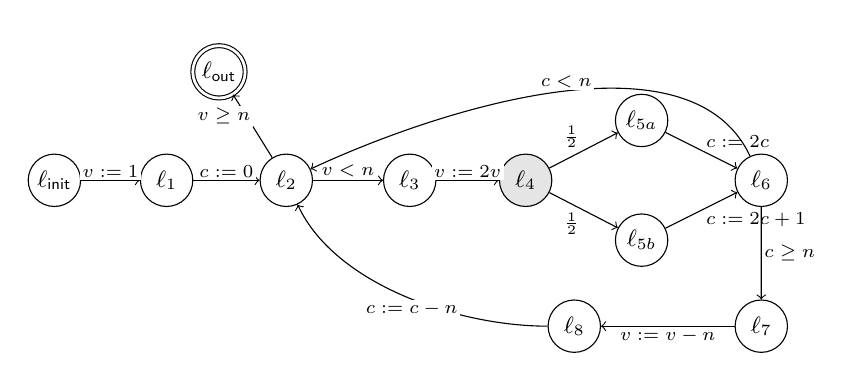
\begin{tikzpicture}[
        ->,
        scale=0.95,
        every node/.style={
            font=\small,
            transform shape
        },
        loc/.style={
            draw,
            circle,
            minimum size=7mm,
            inner sep=1pt
        },
        prob/.style={
            loc,
            fill=black!10
        },
        term/.style={
            loc,
            double,
            double distance=1pt
        },
        lab/.style={
            font=\scriptsize,
            fill=white,
            inner sep=1pt
        }
    ]
        % Initialisation and loop head
        \node[loc]  (init) at (-5.2, 0) {$\ell_{\mathsf{init}}$};
        \node[loc]  (l1)   at (-3.7, 0) {$\ell_1$};
        \node[loc]  (l2)   at (-2.1, 0) {$\ell_2$};

        % Terminal location, moved to the upper left
        \node[term] (out)  at (-3.0, 1.45) {$\ell_{\mathsf{out}}$};

        % Main loop body
        \node[loc]  (l3)   at (-0.45, 0) {$\ell_3$};
        \node[prob] (l4)   at ( 1.10, 0) {$\ell_4$};

        \node[loc]  (l5a)  at (2.65, 0.80) {$\ell_{5a}$};
        \node[loc]  (l5b)  at (2.65,-0.80) {$\ell_{5b}$};

        \node[loc]  (l6)   at (4.25, 0) {$\ell_6$};

        % Rejection branch on a separate lower row
        \node[loc]  (l7)   at (4.25,-1.95) {$\ell_7$};
        \node[loc]  (l8)   at (1.75,-1.95) {$\ell_8$};

        % Initialisation
        \draw (init) --
            node[lab,above] {$v:=1$}
            (l1);

        \draw (l1) --
            node[lab,above] {$c:=0$}
            (l2);

        % Loop guard
        \draw (l2) --
            node[lab,above left,pos=.48] {$v\geq n$}
            (out);

        \draw (l2) --
            node[lab,above] {$v<n$}
            (l3);

        % Deterministic update and probabilistic choice
        \draw (l3) --
            node[lab,above] {$v:=2v$}
            (l4);

        \draw (l4) --
            node[lab,above left,pos=.48] {$\frac12$}
            (l5a);

        \draw (l4) --
            node[lab,below left,pos=.48] {$\frac12$}
            (l5b);

        % Bit-dependent assignments
        \draw (l5a) --
            node[lab,above right,pos=.52] {$c:=2c$}
            (l6);

        \draw (l5b) --
            node[lab,below right,pos=.52] {$c:=2c+1$}
            (l6);

        % Successful iteration: compact upper return
        \draw (l6) to[
            out=115,
            in=25,
            looseness=0.82
        ]
            node[lab,above,pos=.48] {$c<n$}
            (l2);

        % Rejection branch
        \draw (l6) --
            node[lab,right] {$c\geq n$}
            (l7);

        \draw (l7) --
            node[lab,below] {$v:=v-n$}
            (l8);

        % Return after both subtraction assignments
        \draw (l8) to[
            out=180,
            in=-65,
            looseness=0.82
        ]
            node[lab,below,pos=.47] {$c:=c-n$}
            (l2);
    \end{tikzpicture}

    \vspace{-1mm}
    \caption{The pCFG obtained from FDR. The locations
    $\ell_2,\ldots,\ell_8$ expose the loop guard, the update $v:=2v$, the
    fair-bit choice, the bit-dependent updates of $c$, and the rejection
    branch.}
    \label{fig:fdr-pcfg}
\end{figure}


The pCFG rule of Majumdar and Sathiyanarayana is applicable to FDR and
establishes the same AST statement as \Cref{thm:fdr}.  Unlike the
program-level proof, however, it reasons about individual configurations
$(\ell,\sigma)$ of the graph in \Cref{fig:fdr-pcfg}.  Thus, the initialisation,
loop guard, doubling of $v$, fair-bit choice, conditional, and the two
subtraction assignments all become separate proof obligations.

We spell out the pCFG certificate with explicit integrality, parity,
and sublevel bounds. Write
$\mathit{Inv}_\ell$ for the states admitted at location $\ell$. The variable $n$ is integer-valued throughout; $v$ is integer-valued
from $\ell_1$ onward and $c$ from $\ell_2$ onward. Variables not yet
initialized may have arbitrary values.  The invariant
is obtained by transporting the support information
\eqref{eq:fdr-support} through the intermediate assignments:
In this display, $n,v,c$ abbreviate the respective coordinates of $\sigma$.
\begin{align*}
 \mathit{Inv}_{\ell_{\mathsf{init}}}
   &\coloneqq \{\sigma \mid n\in\mathbb{N}_{>0}\},\\
 \mathit{Inv}_{\ell_1}
   &\coloneqq \{\sigma \mid n\in\mathbb{N}_{>0}
                    \land v=1\},\\
 \mathit{Inv}_{\ell_2}
   &\coloneqq \{\sigma \mid n\in\mathbb{N}_{>0}
                    \land 1\leq v<2n
                    \land 0\leq c<\min\{v,n\}\},\\
 \mathit{Inv}_{\ell_3}
   &\coloneqq \{\sigma\in\mathit{Inv}_{\ell_2}\mid
                    v<n\},\\
 \mathit{Inv}_{\ell_4}
   &\coloneqq \{\sigma \mid n\in\mathbb{N}_{>0}
                    \land v\in2\mathbb N_{>0}
                    \land 2\leq v\leq2n-2
                    \land 0\leq c<\tfrac{v}2\},\\
 \mathit{Inv}_{\ell_{5a}}
   &\coloneqq \mathit{Inv}_{\ell_4},
 \qquad
 \mathit{Inv}_{\ell_{5b}}
   \coloneqq \mathit{Inv}_{\ell_4},\\
 \mathit{Inv}_{\ell_6}
   &\coloneqq \{\sigma \mid n\in\mathbb{N}_{>0}
                    \land 2\leq v\leq2n-2
                    \land 0\leq c<v\},\\
 \mathit{Inv}_{\ell_7}
   &\coloneqq \{\sigma\in\mathit{Inv}_{\ell_6}\mid
                   c\geq n\},\\
 \mathit{Inv}_{\ell_8}
   &\coloneqq \{\sigma \mid n\in\mathbb{N}_{>0}
                    \land 1\leq v\leq n-2
                    \land n\leq c<v+n\},\\
 \mathit{Inv}_{\ell_{\mathsf{out}}}
   &\coloneqq \{\sigma\in\mathit{Inv}_{\ell_2}\mid
                    v\geq n\}.
\end{align*}
Hence
\[
    \mathit{Inv}
    \coloneqq
    \bigcup_{\ell}
    \bigl(\{\ell\}\times\mathit{Inv}_{\ell}\bigr)
\]
where $\ell$ ranges over the locations of \Cref{fig:fdr-pcfg},
is an inductive pCFG invariant. The loop-head component
$\mathit{Inv}_{\ell_2}$ is precisely the support part of the distributional
invariant reused in the program-level proof; the other components are
location-specific consequences of it.

The supermartingale is simple but already location-dependent through the
terminal location:
\[
    V(\ell,\sigma)
    \coloneqq
    \begin{cases}
        0, & \ell=\ell_{\mathsf{out}},\\
        \sigma(n), & \ell\neq\ell_{\mathsf{out}}.
    \end{cases}
\]
Since $n$ is never modified, every nonterminal deterministic successor has
the same $V$-value as its predecessor, while a transition to
$\ell_{\mathsf{out}}$ decreases it to $0$.  At the sole probabilistic location
$\ell_4$, both successors retain the value $\sigma(n)$.  Thus the
supermartingale obligations are immediate.  At nonterminal locations, $V\leq r$ implies $n\leq r$. Terminal
states may have arbitrary $n$, but their variant will be zero.

The pCFG variant must instead account for the exact point within an iteration.
The affine certificates of \eqref{eq:fdr-affine-certificates} can also
be extended to pCFG certificates using \Cref{sec:metatheory}.
Here we spell out a location-specific refinement of the logarithmic
alternative \eqref{eq:fdr-log-variant}, based on the iteration-level
distance bound $\left\lceil\log_2\!\bigl(n/(v-c)\bigr)\right\rceil$:
\[
U(\ell,\sigma)\coloneqq
\begin{cases}
  7\left\lceil\log_2(\sigma(n))\right\rceil+3,
    & \ell=\ell_{\mathsf{init}},\\[2pt]
  7\left\lceil\log_2(\sigma(n))\right\rceil+2,
    & \ell=\ell_1,\\[2pt]
  7\left\lceil
      \log_2\!\left(\dfrac{\sigma(n)}{\sigma(v)-\sigma(c)}\right)
    \right\rceil+1,
    & \ell=\ell_2,\\[8pt]
  7\left\lceil
      \log_2\!\left(\dfrac{\sigma(n)}{\sigma(v)-\sigma(c)}\right)
    \right\rceil,
    & \ell=\ell_3,\\[8pt]
  7\left\lceil
      \log_2\!\left(
        \dfrac{\sigma(n)}{\frac{\sigma(v)}2-\sigma(c)}
      \right)
    \right\rceil-1,
    & \ell=\ell_4,\\[10pt]
  7\left\lceil
      \log_2\!\left(
        \dfrac{\sigma(n)}{\sigma(v)-2\sigma(c)}
      \right)
    \right\rceil+5,
    & \ell=\ell_{5a},\\[10pt]
  7\left\lceil
      \log_2\!\left(
        \dfrac{\sigma(n)}{\sigma(v)-(2\sigma(c)+1)}
      \right)
    \right\rceil+5,
    & \ell=\ell_{5b},\\[10pt]
  7\left\lceil
      \log_2\!\left(\dfrac{\sigma(n)}{\sigma(v)-\sigma(c)}\right)
    \right\rceil+4,
    & \ell=\ell_6,\\[10pt]
  7\left\lceil
      \log_2\!\left(\dfrac{\sigma(n)}{\sigma(v)-\sigma(c)}\right)
    \right\rceil+3,
    & \ell=\ell_7,\\[10pt]
  7\left\lceil
      \log_2\!\left(
        \dfrac{\sigma(n)}{\sigma(v)+\sigma(n)-\sigma(c)}
      \right)
    \right\rceil+2,
    & \ell=\ell_8,\\[10pt]
  0,
    & \ell=\ell_{\mathsf{out}}.
\end{cases}
\]

The factor $7$ bounds the number of pCFG transitions needed for one source-level
loop iteration.  The additive offsets ensure strict descent on transitions
that merely change the control location.  The expressions at
$\ell_4,\ell_{5a},\ell_{5b}$ additionally compensate for the fact that one of
the two updates of the iteration has already been executed.  For example,
at $\ell_4$ the current value of $v$ has already been doubled whereas $c$
still has its old value, explaining the denominator
$\sigma(v)/2-\sigma(c)$.  At $\ell_{5a}$ and $\ell_{5b}$, the expressions anticipate the
respective updates of $c$, which are executed on the outgoing edges.
The deterministic decrease conditions can consequently be discharged by
checking the edges of \Cref{fig:fdr-pcfg}; the guard edge to
$\ell_{\mathsf{out}}$ decreases to $0$, and the offsets enforce strict
decrease on the remaining deterministic edges.  At $\ell_4$, the
$\ell_{5a}$ successor---corresponding to the fair-bit outcome $0$---has a
strictly smaller variant.  This successor has probability $\frac12$.
Semantically, this is the familiar iteration-level observation that choosing
the zero bit doubles $v-c$; the rejection updates subtract $n$ from both
variables and hence preserve that difference.  In the pCFG proof this single
observation is distributed over the locations
$\ell_4,\ell_{5a},\ell_6,\ell_7,\ell_8$.

For clarity, the deterministic differences $U_{\rm source}-U_{\rm target}$
are listed below; the state updates on each edge are applied before
computing the target value. Evenness at $\ell_4,\ell_{5a},\ell_{5b}$
ensures $v-(2c+1)\geq1$, so every logarithm is defined.
\begin{center}
\begin{tabular}{@{}ll@{}}
\toprule
Edge & Decrease in $U$\\
\midrule
$\ell_{\mathsf{init}}\to\ell_1$, $\ell_1\to\ell_2$ & $1$\\
$\ell_2\to\ell_3$, $\ell_3\to\ell_4$ & $1$\\
$\ell_{5a}\to\ell_6$, $\ell_{5b}\to\ell_6$ & $1$\\
$\ell_6\to\ell_2$ & $3$\\
$\ell_6\to\ell_7$, $\ell_7\to\ell_8$, $\ell_8\to\ell_2$ & $1$\\
$\ell_2\to\ell_{\mathsf{out}}$ & at least $1$\\
\bottomrule
\end{tabular}
\end{center}
At the fair choice, put
$q=\lceil\log_2(n/(v/2-c))\rceil$.
The zero-bit successor has value $7(q-1)+5=7q-2$, whereas the source
has value $7q-1$. Thus this edge decreases $U$ by one with mass $1/2$;
no descent claim is needed for the other probabilistic edge.

Finally, for $r\geq1$ and a nonterminal configuration with $V\leq r$,
all displayed logarithmic terms are bounded above by
$\lceil\log_2 n\rceil$, using integrality and evenness at $\ell_4$.
Consequently $U\leq7\lceil\log_2r\rceil+5$ suffices.
The initialization values obey the same bound; terminal values are zero,
also when $n>r$. For $r<1$ the sublevel contains only terminal
configurations. Thus the pCFG rule applies with $\varepsilon_r=1/2$.

In comparison, the program-level proof uses the support invariant
$I_{\mathrm{FDR}}$, the affine functions in
\eqref{eq:fdr-affine-certificates} or the logarithmic alternative in
\eqref{eq:fdr-log-variant}, and the single body calculation
\eqref{eq:fdr-post}. It retains the support information from the
uniform-output invariant. Both proof routes have the same proving power, but the
program-level rule expresses the algorithmic fact---progress over a complete
loop iteration---without introducing locations, offsets, and intermediate
state expressions solely for control-flow bookkeeping.


\section{Synthesis Details and Artifact Checks}
\label[appendix]{app:artifact}

This appendix provides the search procedure, model encodings, and
additional checks underlying \Cref{tab:synthesis-results}.

\subsection{Search Procedure and Supplied Partitions}
\label[appendix]{app:synthesis-search}

Before searching, Z3 checks initial inclusion in $S$ and preservation
by each represented outcome. For an abstraction it also checks
$S\land b\Rightarrow\exists\xi\,A(\sigma,\xi)$, so every enabled
state admits an outcome description. This last query may be quantified.

Fix a coefficient bound $B$. Each unknown coefficient is an integer
between $-B$ and $B$. The search proceeds as follows:
\begin{enumerate}
 \item \emph{Choose a sample.} Z3 selects an enabled state in $S$
 and, if needed, an admissible $\xi$. If none exists, all initial
 states are already terminal.
 \item \emph{Propose coefficients.} The learner chooses both vectors
 so that all verification conditions hold on the accumulated samples.
 It minimizes the sum of absolute coefficient values to favor small
 expressions; this objective has no soundness role.
 \item \emph{Check all states.} With coefficients fixed, the verifier
 searches for an enabled state and admissible $\xi$ violating a condition.
 A counterexample is added to the samples before returning to the learner.
 \item \emph{Accept a verified pair.} An unsatisfiable verifier query
 establishes the conditions over the entire invariant domain, including
 unbounded integer inputs. The implementation accepts the pair after
 also checking each condition separately.
\end{enumerate}
The learner and verifier alternate which quantities are fixed.
On a fixed sample, the constraints are linear in the unknown template
coefficients. With coefficients fixed, they are Boolean combinations
of linear arithmetic in the state and auxiliary transition variables
for the supported encodings. The verification domain is never bounded
by the coefficient bound $B$.

Each counterexample excludes the current candidate and no valid one.
Thus exact terminating solvers, without resource limits, decide existence
within each finite coefficient set. The implementation tries
$B=1,2,4,8,16$, retaining samples between bounds. Learner unsatisfiability
excludes only the current bound; exhausting the schedule excludes only
the tested coefficient sets. Unknown results, timeouts, and the limit of 500
candidates are inconclusive and retain the available search context.
Relative completeness of the rule does not imply completeness of this
search: templates, domination, and a possibly overapproximating supplied
invariant can each exclude otherwise available certificates.

\paragraph{Fixed piecewise affine templates.}
The same procedure accepts a supplied finite partition
$P_1,\ldots,P_q$ of the enabled states in $S$.
It checks that the regions cover this domain and are pairwise disjoint,
then creates a separate affine coefficient block for each region and
each certificate. For example, the supermartingale template is
\[
 V(\sigma)=[b](\sigma)\sum_{j=1}^{q}[P_j](\sigma)
 \left(a_{j,0}+\sum_{i=1}^{d}a_{j,i}x_i(\sigma)\right).
\]
The variant template has its own coefficient blocks.
The partition predicates are supplied Boolean combinations of linear
arithmetic over declared state components, including symbolic program
inputs. They cannot depend on template coefficients or auxiliary
transition variables. The verifier evaluates the partition again at
each successor, so it also checks transitions between regions.
The verification conditions and their soundness argument are unchanged.

The algorithm searches for coefficients, not partition predicates or
thresholds. The two-sided walk in \Cref{app:synthesis-models} illustrates their
benefit; \Cref{app:synthesis-checks} gives optional sampler splits.

\subsection{Loop Models and Certificate Analysis}
\label[appendix]{app:synthesis-models}

The following models instantiate the common interface of
\Cref{sec:synthesis-constraints}. All displayed certificate expressions
are their values on enabled states; guarded templates assign zero on
terminal states.

\paragraph{Unbounded symmetric random walk.}
For the random walk in \Cref{sec:rule-examples}, the model has $S\equiv x\geq0$, guard
$x>0$, and the equally likely updates $x\mapsto x-1$ and $x\mapsto x+1$.
The engine constructs the basis $(x,1)$ and finds $V=U=x$ on enabled
states, verified without an upper bound on $x$. The expectation is
unchanged, while the left outcome decreases $U$ by one.
This establishes AST despite infinite expected runtime:
for $0<x<N$, the expected time $x(N-x)$ to hit $\{0,N\}$ lower-bounds
the expected time to hit $0$, and diverges with $N$.
A uniform negative expected drift is unnecessary.

\paragraph{FDR with a symbolic range.}
For the loop of \Cref{sec:fdr}, the supplied invariant is
$S\equiv n\geq1\land1\leq v<2n\land0\leq c<v\land c<n$, and the
complete bit-$\beta$ update is
\[
 T_\beta(n,v,c)=
 \begin{cases}
 (n,2v-n,2c+\beta-n),&2c+\beta\geq n,\\
 (n,2v,2c+\beta),&2c+\beta<n.
 \end{cases}
\]
Here $n$ is a read-only program input. From the declared integer
components the engine constructs the full basis $(n,v,c,1)$ and finds
$V=n$, $U=n-v+c$ on $v<n$, verified for all admitted values of $n$.
This recovers the affine certificates of \Cref{thm:fdr}.
Writing $\Delta=v-c\geq1$, the identity $\Delta'=2\Delta-\beta$
also yields $\mathbb E[U']\leq U-1/2$: bit zero decreases $U$ by
at least one, and bit one does not increase it; acceptance sets it to zero.
This stronger inequality is independently SMT-verified, so $U$ is itself
a ranking supermartingale.

\paragraph{FLDR with fixed weights.}
For $(4,5)$, preprocessing gives $m=9$, $k=4$, and rejection weight $7$.
The artifact constructs the exact tree using the row convention of
\Cref{sec:fldr}. Its loop-head nodes form the invariant, internal nodes
satisfy the guard, and the bit edges include resets. Since $m,k,n$ are
fixed numerical values, the integer state components are $c,d$, giving
the basis $(c,d,1)$. After excluding $B=1$, it finds
$V=U=c-2d+2$ at $B=2$. \Cref{fig:fldr-synthesis-tree} displays the
five active nodes, acceptances, and resets. An independent rational-arithmetic
audit checks all nodes and edges (\Cref{app:synthesis-checks}). At the root the
expectation is unchanged, so this shared certificate has no uniformly
negative expected change.
\begin{figure}[tbp]
 \centering
 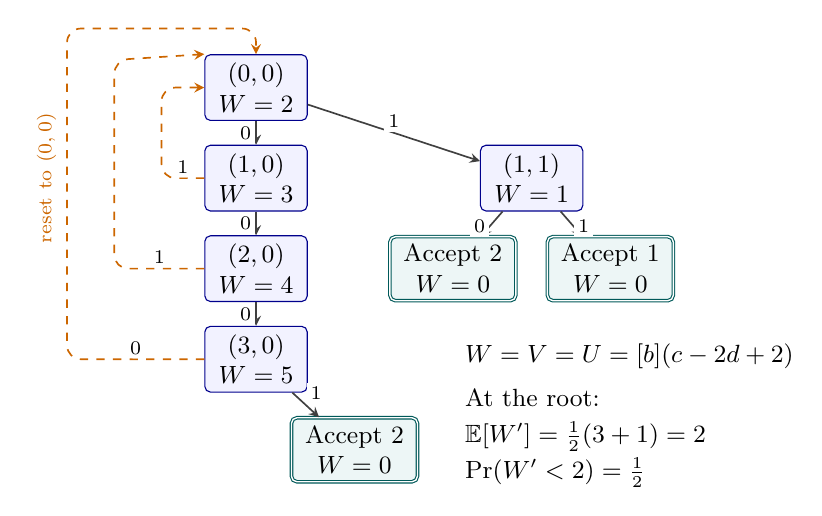
\begin{tikzpicture}[
   x=1cm,y=1cm,>=stealth,
   fldrnode/.style={draw=blue!55!black,fill=blue!5,rounded corners=2pt,
     minimum width=13mm,minimum height=8mm,inner sep=3pt,
     align=center,font=\small},
   fldraccept/.style={draw=teal!70!black,fill=teal!7,
     double,double distance=.5pt,rounded corners=2pt,
     minimum width=16mm,inner sep=3pt,align=center,font=\small},
   fldredge/.style={->,semithick,draw=black!75},
   fldrreset/.style={->,semithick,dashed,draw=orange!80!black,
     rounded corners=5pt},
   fldrbit/.style={font=\scriptsize,fill=white,inner sep=1.5pt}
 ]
 \node[fldrnode] (root) at (0,0) {$(0,0)$\\$W=2$};
 \node[fldrnode] (s10) at (0,-1.15) {$(1,0)$\\$W=3$};
 \node[fldrnode] (s11) at (3.5,-1.15) {$(1,1)$\\$W=1$};
 \node[fldrnode] (s20) at (0,-2.30) {$(2,0)$\\$W=4$};
 \node[fldrnode] (s30) at (0,-3.45) {$(3,0)$\\$W=5$};
 \node[fldraccept] (a22) at (2.5,-2.30)
   {Accept $2$\\$W=0$};
 \node[fldraccept] (a23) at (4.5,-2.30)
   {Accept $1$\\$W=0$};
 \node[fldraccept] (a41) at (1.25,-4.60)
   {Accept $2$\\$W=0$};

 % Each arrow includes every update of one loop-body execution.
 \draw[fldredge] (root) -- node[fldrbit,left] {$0$} (s10);
 \draw[fldredge] (root) -- node[fldrbit,above] {$1$} (s11);
 \draw[fldredge] (s10) -- node[fldrbit,left] {$0$} (s20);
 \draw[fldredge] (s11) -- node[fldrbit,pos=.58,left] {$0$} (a22);
 \draw[fldredge] (s11) -- node[fldrbit,pos=.58,right] {$1$} (a23);
 \draw[fldredge] (s20) -- node[fldrbit,left] {$0$} (s30);
 \draw[fldredge] (s30) -- node[fldrbit,above right] {$1$} (a41);

 % Reset events are contracted into their bit-labelled body transitions;
 % raw rejecting leaves are not loop-head states and get no certificate value.
 \draw[fldrreset] (s10.west) -- node[fldrbit,above] {$1$}
   (-1.20,-1.15) -- (-1.20,0) -- (root.west);
 \draw[fldrreset] (s20.west) -- node[fldrbit,above] {$1$}
   (-1.80,-2.30) -- (-1.80,.35) -- (root.north west);
 \draw[fldrreset] (s30.west) -- node[fldrbit,above] {$0$}
   (-2.40,-3.45) -- (-2.40,.75) -- (0,.75) -- (root.north);
 \node[font=\scriptsize,text=orange!80!black,rotate=90]
   at (-2.66,-1.15) {reset to $(0,0)$};

 \node[align=left,font=\small,anchor=north west,inner sep=0pt]
   at (2.65,-3.25)
   {$W=V=U=[b](c-2d+2)$\\[5pt]
    At the root:\\[2pt]
    $\mathbb E[W']=\tfrac12(3+1)=2$\\[2pt]
    $\Pr(W'<2)=\tfrac12$};
 \end{tikzpicture}
 \caption{A decision tree for FLDR with weights $(4,5)$ and rejection
 weight $7$. Active nodes show $(c,d)$ and the shared certificate value
 $W$; double-bordered leaves accept the indicated outcome and have value
 zero. Every edge represents one complete iteration with probability
 $1/2$; its label is the sampled bit. Dashed edges include rejection and
 reset, returning to the root with $W=2$. The root calculation illustrates
 progress despite zero expected decrease.}
 \label{fig:fldr-synthesis-tree}
\end{figure}

\paragraph{FLDR with symbolic inputs and abstract outcomes.}
To cover arbitrary FLDR weight vectors without constructing every tree,
we supply an abstraction of the body outcomes. Its integer components
are $(m,k,n,c,d)$, with read-only inputs $m,k,n$; a Boolean flag
$\mathit{active}$ is the guard. The supplied invariant requires
$m\geq1$, $0\leq k\leq m$, $1\leq n\leq m$, $0\leq c\leq k$,
$d\geq0$, and $\mathit{active}\Rightarrow c<k$.
The auxiliary transition description is $\xi=(t_0,t_1)$, where each
$t_\beta\in\{0,1,2\}$ classifies the outcome of bit $\beta$ as
continuation, rejection, or acceptance, respectively.
Continuation advances to $(c+1,2d+\beta)$ and requires $c+1<k$;
rejection resets to $(0,0)$; acceptance advances to the child and
disables the guard. Continuation and rejection leave the guard enabled.
The inputs $m,k,n$ are unchanged. The relation $A(\sigma,\xi)$ excludes
$(t_0,t_1)=(1,1)$, so at least one outcome does not reject.

Tree height at most $k$ and at most one rejecting leaf per level justify
this abstraction of concrete FLDR executions (\Cref{sec:fldr}).
The certificate solver does not derive these facts from preprocessing.
The linear domain relaxes $k=\lceil\log_2m\rceil$ to $0\leq k\leq m$,
avoiding logarithmic arithmetic. From all integer components, the engine
constructs the basis $(m,k,n,c,d,1)$ and finds $V=m$, $U=k-c$ on active
states. The unused features remain in the templates; their coefficients are
synthesized as zero.
Every successor has $V'$ equal to $m$ or zero, a nonrejecting outcome
decreases $U$ by at least one, and $1\leq U=k-c\leq k\leq m=V$.
The alternative pair $V=k$, $U=k-c$ is also independently verified,
but is not the candidate selected in the recorded affine run.
Verification ranges over all pairs admitted by $A$, including pairs
absent from any particular fixed tree. This larger domain explains why
the concrete and abstract certificates may differ.

The depth variant can grow in expectation: at $(c,d)=(2,0)$ in the
fixed tree, $U=2$ but $\mathbb E[U']=5/2$. The separate supermartingale
still satisfies its bound. This does not establish an intrinsic need for
distinct functions: the concrete certificate $c-2d+2$ serves both roles.
\Cref{app:synthesis-checks} explains the obstruction only for depth-only affine
shared functions.

\paragraph{What the supplied partition adds.}
For the symmetric walk on all of $\mathbb Z$, the supplied model has
guard $x\neq0$, invariant $S\equiv\mathit{true}$, and the two equally
likely updates $x\mapsto x-1$ and $x\mapsto x+1$.
An affine variant $ax+b$ positive on both unbounded
tails must have $a=0$, and a constant cannot decrease at $x=2$. Hence no
single-affine pair satisfies the constraints, regardless of its coefficient
bound. With the supplied split $x<0$ versus $x\geq0$, the same engine
synthesizes the expressions $-x$ and $x$ for the respective regions in
both templates, giving the universally verified pair $V=U=|x|$.
Thus a supplied partition makes a certificate expressible that no
single-affine template can represent on this invariant.

\subsection{Reproducing the Experiments and Additional Checks}
\label[appendix]{app:synthesis-checks}

The companion package implements the constraints of
\Cref{sec:certificate-synthesis}. It trusts the supplied semantic encoding,
the mathematical FLDR abstraction argument, and Z3's answers.
Supplied invariants are checked for initialization and preservation
against that encoding.
It neither mechanizes the metatheory nor independently checks solver proof
objects. The README gives file-level documentation, exact commands, and
expected results. The shared kernel is in \texttt{engine.py};
\texttt{examples.py} supplies inputs and the finite FLDR tree constructor.
From the artifact directory, run:
\begin{lstlisting}[basicstyle=\ttfamily\small,breaklines=true]
python3 -m pip install -r requirements.txt
python3 synthesis_examples.py --output run.json
python3 diagnostics.py --output checks.json
python3 audit_sampler_certificates.py --output audit.json
\end{lstlisting}
The recorded synthesis run in \texttt{results.json} uses
Python~3.13.0/Z3~4.15.4 and verifies all eight positive inputs.
JSON files record coefficients, counterexamples, individual
obligation checks, bounds, and measured wall times. Solver-selected
certificates, candidate counts, and timings may vary across systems. No performance
comparison is claimed. Failure of
the unpartitioned two-sided walk excludes only the tested bounds; the
all-bounds impossibility is proved analytically in
\Cref{app:synthesis-models}.

Unknown solver results and resource limits are reported as inconclusive,
including in the negative experiment. The JSON retains the solver reason,
phase, current coefficient bound, samples, candidate trace, and completed
checks whenever available. A pair is marked verified only after all
individual rechecks succeed. Any inconclusive experiment makes the runner
exit with nonzero status, even if all positive inputs were verified.

\paragraph{Optional partitions and negative checks.}
For the optional sampler splits the caller supplies both predicates:
$2v<n$ and $2v\geq n$, or $c<k-1$ and $c\geq k-1$.
The latter expression depends on the read-only input $k$; its syntax is
fixed, although the numerical threshold varies between inputs.
Only coefficients within the regions are synthesized.
The successful coefficient bounds are $1,2,1$ for FDR, fixed FLDR,
and abstract FLDR, respectively. The recorded fixed-tree certificate uses $c-2d+2$
below depth $3$ and the constant $1$ at depth $3$. Abstract FLDR uses $V=k$ and
$U=k-c$, represented by $1$ in the final active region. No extra split
is necessary for the baseline sampler results.

Diagnostics reject invalid certificates, a vacuous transition contract,
and overlapping, incomplete, or ill-scoped partitions. A signed countdown
crosses the partition boundary in both directions and verifies $|x|$
universally. The FDR drift inequality and alternative abstract pair
$V=k$, $U=k-c$ are separately SMT-checked.

\paragraph{The depth-only shared-template obstruction.}
In the fixed FLDR tree for $(4,5)$, suppose a shared affine function
omits the node index $d$. At $k=4$ it has the enabled expression
$W(c)=A+Dc$. Both root successors have depth one, so progress forces
$D<0$. At $(c,d)=(2,0)$ the successors have depths three and zero,
giving expected change $-D/2>0$, contrary to the supermartingale
condition. The full template includes $d$ and admits $c-2d+2$.
The obstruction therefore concerns only this restricted template class.

\paragraph{An exact audit of the concrete FLDR certificate.}
For weights $(4,5)$ the shared certificate $W=c-2d+2$ gives:
\begin{center}
\begin{tabular}{@{}ccccc@{}}
\toprule
$(c,d)$ & $W$ & Successor values & Mean & A strict decrease\\
\midrule
$(0,0)$ & $2$ & $(3,1)$ & $2$ & $2\to1$\\
$(1,0)$ & $3$ & $(4,2)$ & $3$ & $3\to2$\\
$(1,1)$ & $1$ & $(0,0)$ & $0$ & $1\to0$\\
$(2,0)$ & $4$ & $(5,2)$ & $7/2$ & $4\to2$\\
$(3,0)$ & $5$ & $(2,0)$ & $1$ & $5\to0$\\
\bottomrule
\end{tabular}
\end{center}
The diagnostic checks these rows with integers and rational numbers,
independently of SMT solving. Both certificates are positive integers on
active nodes and zero on terminal nodes. Each mean is at most the current
value and each pair has a smaller value, with probability at least $1/2$.
Domination follows from $U=V$.

\paragraph{Finite preprocessing and sampler audits.}
Exact arithmetic checks all 1,554 weight vectors with one to four outcomes
and weights in $\{1,\ldots,6\}$. These tests validate dyadic leaf masses,
height, reset targets, the structural contract, $d<2n$, and immediate
root acceptance. They support the universal row argument in
\Cref{app:calculations}, but do not replace it. An independent diagnostic
additionally checks 247,721 FDR location-states with $n\leq40$ and
11,424 Han--Hoshi intervals across 84 weight vectors. Its JSON specifies
the finite domains.

These checks have distinct scopes: universal SMT validation on supplied
domains, exact enumeration of a fixed tree, and bounded regression across
instances. No simulation estimate is used as a certificate or as a proof
of AST.

\fi

\end{document}
